\documentclass[12pt, a4paper, onecolumn, oneside, final]{report}

%%========================================================================
%% WAJIB DIISI SESUAI DATA YANG BENAR DAN TIDAK BOLEH ADA YANG TERLEWAT
%%========================================================================

\providecommand{\judulid}{Analisis Performa Quadcopter dengan Penerapan Algoritma Kendali Pid pada Kontroler Penerbangan blablabla blablabla blablabla blablabla blablabla} %Judul Tugas Akhir Bahasa Indonesia
\providecommand{\judulen}{Quadcopter Performance Analysis with the Application of the Pid Control Algorithm on the Flight Controller blablabla blablabla blablabla blablabla blablabla} %Judul Tugas Akhir Bahasa Inggirs
\providecommand{\penulis}{Bintang Chen Sudiro Hutama Karya} %Nama Lengkap Mahasiswa 
\providecommand{\nim}{10293847564738} % NIM

\providecommand{\tipe}{Proyek Akhir} %Tipe Laporan
\providecommand{\type}{Final Project} %Tipe Laporan
\providecommand{\prodi}{Sarjana Terapan Teknik Elektronika} %Nama Prodi
\providecommand{\fakultas}{Fakultas Vokasi} %Nama Fakultas
\providecommand{\universitas}{Universitas Negeri Yogyakarta} %Nama Universitas

\providecommand{\tglpersetujuan}{\today} %Tanggal di Lembar Persetujuan
\providecommand{\tglpernyataan}{\today} %Tanggal di Surat Pernyataan
\providecommand{\tglpengesahan}{\today} %Tanggal di Halaman Pengesahan
\providecommand{\tahun}{\the\year{}} %Tahun Proyek Akhir

\providecommand{\sekretaris}{Nama Sekretaris} %Nama Sekretaris Penguji
\providecommand{\penguji}{Nama Penguji} %Nama Penguji
\providecommand{\dekan}{Dr. Komarudin, S.Pd., M.A.} %Nama Dekan
\providecommand{\NIPdekan}{197409282003121002} %NIP Dekan

\providecommand{\koorprodi}{Dr. Aris Nasuha, S.Si., M.T.} %Nama Koorprodi
\providecommand{\NIPkoorprodi}{196906151994031002} %NIP Koorprodi

\providecommand{\pembimbing}{Nama Dosen Pembimbing} %Nama Dosen Pembimbing
\providecommand{\NIPpembimbing}{123456789012345678} %NIP Dosen Pembimbing

\providecommand{\katakunci}{Konsep Abstrak, Komponen Abstrak, Kata Kunci.} %Kata kunci dalam Bahasa Indonesia
\providecommand{\keywords}{Abstract Concepts, Abstract Components, Key Words.} %Kata kunci dalam Bahasa Inggris
<<<<<<< HEAD
%%File ini adalah file konfigurasi, tidak perlu diubah kecuali paham dengan apa yang ditambahkan

%pengaturan margin
\usepackage{geometry}
\geometry{verbose,tmargin=3cm,bmargin=3cm,lmargin=4cm,rmargin=3cm}

%paket bahasa indonesia
%\usepackage[bahasa]{babel}
% Mengatur bahasa latex
\usepackage[indonesian]{babel}
\usepackage[utf8]{inputenc}

%direktor penyimpanan gambar
\usepackage{graphicx}
\graphicspath{{gambar/}}

%paket untuk tabel
\usepackage{tabularx}

%paket untuk mengatur space
\usepackage{setspace}
\onehalfspacing

% Untuk mengatur spacing antara paragraf
\usepackage{parskip}

% Membuat indent
\usepackage{indentfirst}
\setlength\parindent{1cm}

% Membuat seluruh tulisan menjadi Times New Roman. 
\usepackage{pslatex}

%pentauran font
\usepackage[T1]{fontenc}
%\usepackage{times}

% Mengatur font section
\usepackage{sectsty}
\sectionfont{\fontsize{12}{14}\selectfont}
\subsectionfont{\fontsize{12}{14}\selectfont}
\subsubsectionfont{\fontsize{12}{14}\selectfont}

%menambahkan titik titik di daftar isi, gambar, tabel
\usepackage{tocloft}
%\renewcommand{\cftdot}{\textperiodcentered}
%\renewcommand{\cftchapdotsep}{\cftdotsep}
%\renewcommand{\cftpartleader}{\cftdotfill{\cftdotsep}}
%\renewcommand{\cftchapleader}{\cftdotfill{\cftdotsep}}
%\renewcommand{\cftsecleader}{\cftdotfill{\cftdotsep}}
%\usepackage[subfigure]{tocloft}
%\renewcommand{\cftpartleader}{\dotfill}
%\renewcommand{\cftpartafterpnum}{\cftparfillskip}
%\renewcommand{\cftchapleader}{\dotfill}
%\renewcommand{\cftsecleader}{\dotfill}
%\renewcommand{\cftsubsecleader}{\dotfill}


%tambah "bab" x di daftar isi 
\renewcommand*\cftchappresnum{\MakeUppercase{bab}~}
\renewcommand\chaptername{BAB}
\settowidth{\cftchapnumwidth}{\cftchappresnum}
\renewcommand{\cftchapaftersnumb}{\quad}
\addtocontents{toc}{
    %\renewcommand\protect*\protect\cftchappresnum{\MakeUppercase{\chaptername}~}}
    \protect\renewcommand*\protect\cftchappresnum{\MakeUppercase{\chaptername}~}}

%pengaturan chapter menjadi tengah dan angka romawi
\usepackage{titlesec}
\titleformat{\chapter}[display]
{\normalfont\Large\bfseries\centering}
{\MakeUppercase{\chaptertitlename}\ \Roman{chapter}}
{.5em}
{\MakeUppercase}

%paket untuk bibTex
\usepackage{cite}
\bibliographystyle{IEEEtran}
%==================================================================
% Ini adalah file konfigurasi
%==================================================================

%% DILARANG EDIT BAGIAN INI

% Mengatur bahasa latex
\usepackage[indonesian]{babel}
\usepackage[utf8]{inputenc}

% Untuk pengaturan spacing
\usepackage{setspace}
\onehalfspacing

% Untuk mengatur level section 
\setcounter{secnumdepth}{6}

% Digunakan untuk memasukan gambar ke laporan. 
\usepackage{graphicx}
\graphicspath{{gambar/}}
\usepackage{float}
\usepackage[hang,nooneline,scriptsize,md]{subfigure}
\usepackage[subfigure]{tocloft}

% Untuk mengatur spacing antara paragraf
\usepackage{parskip}

% Membuat indent
\usepackage{indentfirst}
\setlength\parindent{1cm}

% Untuk mengkustomisasi margin
\usepackage{scrextend}

% Untuk mengatur header dan footer
\usepackage{fancyhdr}

% Membuat seluruh tulisan menjadi Times New Roman. 
\usepackage{pslatex}

% Merubah numbering chapter dan section untuk judul setiap bab menggunakan romawi dan judul anak bab menggunakan arabic
\renewcommand{\thesection}{\arabic{chapter}.\arabic{section}\hspace{0.05cm}}
\renewcommand{\thesubsection}{\arabic{chapter}.\arabic{section}.\arabic{subsection}\hspace{-0.25cm}}
\renewcommand{\thesubsubsection}{\arabic{chapter}.\arabic{section}.\arabic{subsection}.\arabic{subsubsection}\hspace{-0,35cm}}

% Mengatur identasi judul section dan subsection
%\titleformat{\section}[block]{\bfseries}{\thesection.}{1em}{}
%\titleformat{\subsection}[block]{\hspace{2em}}{\thesubsection}{1em}{}

% Merubah huruf kapital pada judul daftar isi, daftar gambar, dan daftar table
\usepackage{tocloft}
\renewcommand{\cfttoctitlefont}{\hfil\large\bfseries\MakeUppercase}
\renewcommand{\cftloftitlefont}{\hfil\large\bfseries\MakeUppercase}
\renewcommand{\cftlottitlefont}{\hfil\large\bfseries\MakeUppercase}

\renewcommand\cftchappresnum{BAB }
\renewcommand\cftchapaftersnum{}
\newlength\mylen
\settowidth\mylen{\bfseries BAB 1 :\ } % if more than 9 chapters, use "Chapter 10"
\cftsetindents{chap}{0pt}{\mylen}

% Mengatur font section
\usepackage{sectsty}
\sectionfont{\fontsize{12}{14}\selectfont}
\subsectionfont{\fontsize{12}{14}\selectfont}
\subsubsectionfont{\fontsize{12}{14}\selectfont}

% Untuk merupakan format penulisan BAB
\usepackage{titlesec}
\titleformat{\chapter}
{\doublespacing\fontsize{14pt}{16pt}\bfseries}
{\MakeUppercase{\chaptertitlename\ \Roman{chapter}}\filcenter}
{0.15cm}{\centering\uppercase}
\titlespacing*{\chapter}{0pt}{-1cm}{20pt}

% Mengatur spacing section
\titlespacing*{\section}
{0pt}{10pt}{0cm}
\titlespacing*{\subsection}
{0pt}{10pt}{0cm}
\titlespacing*{\subsubsection}
{0pt}{10pt}{0cm}

% Digunakan untuk mengatur caption dalam dokumen.
\usepackage[font=footnotesize,format=plain,labelfont=bf,up,textfont=up]{caption}

% Untuk menghapus titik dua (colon)
\captionsetup[figure]{labelsep=space}
\captionsetup[table]{labelsep=space}

% Mengatur nomor caption gambar
\renewcommand{\thefigure}{\arabic{chapter}.\arabic{figure}}

% Mengatur nomor caption table
\renewcommand{\thetable}{\arabic{chapter}.\arabic{table}}

% Mengatur Hyphenation pada latex
\tolerance=1
\emergencystretch=\maxdimen
\hyphenpenalty=10000
\hbadness=10000

% Untuk mengatur setting indent
\setlength\parindent{1cm}

% Untuk memasukkan table
\usepackage{tabularx}
\usepackage{multirow}

% Untuk mengatur width
\usepackage{changepage}

% Menggatur setting halaman 
\usepackage{geometry}
\geometry{
    left=4cm,            % <-- you want to adjust this
    top=3cm,
    right=3cm,
    bottom=3cm,
}

% Teks testing
\usepackage{blindtext}
\usepackage{lipsum}

% Untuk mengatur subscript supscript
\usepackage{fixltx2e}

% Untuk mengatur wrap picture
\usepackage{wrapfig}

% Untuk notasi matematika
\usepackage{amsmath}
\usepackage{stmaryrd}
\usepackage{mathtools}

% untuk mengatur label nomor pada rumus
\renewcommand{\theequation}{\arabic{chapter}.\arabic{equation}}

% Untuk mengatur spacing daftar gambar
\newcommand*{\noaddvspace}{\renewcommand*{\addvspace}[1]{}}
\addtocontents{lof}{\protect\noaddvspace}

%untuk mengatur package include table in excel
% \usepackage{pgfplotstable}

% untuk mengatur landscape page
\usepackage{rotating}

% untuk list
\usepackage{enumitem}
\newenvironment{packed_enum}{
    \begin{enumerate}[leftmargin=1.5\parindent]
        \setlength{\itemsep}{0pt}
        \setlength{\parskip}{0pt}
        \setlength{\parsep}{0pt}
        }{\end{enumerate}}

\newenvironment{packed_item}{
    \begin{itemize}[leftmargin=1.5\parindent]
        \setlength{\itemsep}{0pt}
        \setlength{\parskip}{0pt}
        \setlength{\parsep}{0pt}
        }{\end{itemize}}

%paket untuk bibTex
\usepackage{cite}
\bibliographystyle{IEEEtran}

%paket untuk mengembed kode dalam LaTeX
\usepackage{listings}
\lstset{
    basicstyle=\small,
    %basicstyle=\ttfamily,
    columns=fullflexible,
    frame=single,
}

%paket untuk tabel
\usepackage{longtable}

%paket untuk url
\usepackage{hyperref}

% styling python
\usepackage{color}
\usepackage{listings}    
\usepackage{courier}

\definecolor{mygreen}{rgb}{0,0.6,0}
\definecolor{mygray}{rgb}{0.5,0.5,0.5}
\definecolor{mymauve}{rgb}{0.58,0,0.82}

\lstset{ %
  backgroundcolor=\color{white},   % choose the background color
  basicstyle=\footnotesize,        % size of fonts used for the code
  breaklines=true,                 % automatic line breaking only at whitespace
  captionpos=b,                    % sets the caption-position to bottom
  commentstyle=\color{mygreen},    % comment style
  escapeinside={\%*}{*)},          % if you want to add LaTeX within your code
  keywordstyle=\color{blue},       % keyword style
  stringstyle=\color{mymauve},     % string literal style
}
%% DILARANG EDIT BAGIAN INI
\hyphenation{di-la-ku-kan} %bisa dilihat di bagian "abstrak"

%tulis seperlunya, kalau menemukan kata yang terpenggal salah, misalnya.. 
\hyphenation{be-ri-kut}
\hyphenation{a-da-lah} %dsb.. 
\begin{document}
%==================================================================
% Ini adalah sampul luar
%==================================================================

%% DILARANG EDIT BAGIAN INI

\begin{titlepage}
    \begin{center}

        \begin{doublespace}
            \textbf{\Large{\MakeUppercase{\judulid}}}\\[2cm]
        \end{doublespace}
        \textbf{\MakeUppercase{\large{\tipe}}}\\[0.5cm]

        Diajukan kepada {\fakultas} {\universitas} Untuk Memenuhi Sebagai Persyaratan Guna Memperoleh Gelar Sarjana Terapan\\[2cm]
        
\includegraphics[width=0.3\linewidth]{gambar/logo-uny.png}\\[2cm]

        \textbf{Oleh:} \\
        \textbf{\MakeUppercase{{\penulis}}} \\
        \textbf{NIM} \textbf{{\nim}}\\[2cm]

        \vfill

        \textbf{\large \MakeUppercase{Prodi \prodi}}\\
        \textbf{\large \MakeUppercase{\fakultas}}\\
        \textbf{\large \MakeUppercase{\universitas}}\\
        \textbf{\large \the\year{}}\\
    \end{center}
\end{titlepage}

%% DILARANG EDIT BAGIAN INI
\pagenumbering{roman}
%lembar pengesahan
\newpage
%\thispagestyle{empty}
\addcontentsline{toc}{chapter}{HALAMAN SAMPUL}
\begin{center}
    %bagian atas dari halaman
    \begin{doublespace}
        \textbf{\large{\MakeUppercase{\judulid}}}\\[2.5cm]
    \end{doublespace}

    \textbf{\MakeUppercase{\large{\tipe}}}\\[0.5cm]
    \begin{onehalfspace}
        Diajukan kepada {\fakultas} {\universitas} Untuk Memenuhi Sebagai Persyaratan Guna Memperoleh Gelar Sarjana Terapan\\[1.8cm]
    \end{onehalfspace}

    \large Oleh: \\
    \begin{onehalfspace}
        \large{\penulis} \\
        \large{\nim}\\[1.5cm]
    \end{onehalfspace}
    \vspace{1.5cm}

    % EDIT PEMBIMBING, udah deh sampul2. :D
    \large Pembimbing: \\
    \begin{onehalfspace}
        \large{\pembimbing} \\
    \end{onehalfspace}

    \vfill

    % bagian bawah
    \textbf{\large \MakeUppercase{Prodi \prodi}}\\
    \textbf{\large \MakeUppercase{\fakultas}}\\
    \textbf{\large \MakeUppercase{\universitas}}\\
    \textbf{\large \the\year{}}\\
\end{center}

%==================================================================
% Ini adalah halaman persetujuan
%==================================================================

%% DILARANG EDIT BAGIAN INI
\newpage
\addcontentsline{toc}{chapter}{LEMBAR PERSETUJUAN}
\begin{center}
    \begin{doublespace}
        \textbf{\large \MakeUppercase{lembar persetujuan}}
    \end{doublespace}
\end{center}

\begin{center}
    {\tipe} dengan Judul
\end{center}

\begin{center}
    \begin{doublespace}
        \textbf{\large \MakeUppercase {\judulid}}
    \end{doublespace}
\end{center}

\begin{center}
    Disusun oleh:\\
    \textbf{\penulis}\\
    \textbf{NIM \nim}\\[1.5cm]

    telah memenuhi syarat dan disetujui oleh Dosen Pembimbing untuk dilaksanakan Ujian {\tipe} bagi yang bersangkutan.\\[0.75cm]
\end{center}

\begin{minipage}{0.35\textwidth}
    \hfill\\[2em]
    Mengetahui,\\
    Koordinator Program Studi,\\[2cm]
    \koorprodi\\
    NIP. \NIPkoorprodi
\end{minipage}
\hfill
\begin{minipage}{0.35\textwidth}
    Wates, \tglpersetujuan\\[1em]
    Disetujui,\\
    Dosen Pembimbing TA,\\[2cm]
    \pembimbing\\
    NIP. \NIPpembimbing
\end{minipage}%
%% DILARANG EDIT BAGIAN INI
%==================================================================
% Ini adalah surat pernyataan
%==================================================================

%% Edit sesuai kebutuhan
\newpage
\addcontentsline{toc}{chapter}{SURAT PERNYATAAN}
\begin{center}
    \begin{doublespace}
        \textbf{\large \MakeUppercase{surat pernyataan}}
    \end{doublespace}
\end{center}

\noindent Saya yang bertandatangan di bawah ini saya:

\begin{table}[h!]
    \begin{tabular}{lll}
        Nama              & : & \penulis \\
        NIM               & : & \nim     \\
        Program Studi     & : & \prodi   \\
        Judul Tugas Akhir & : & \judulid
    \end{tabular}
\end{table}

\noindent menyatakan bahwa tugas akhir ini benar-benar karya saya sendiri*). Sepanjang pengetahuan saya tidak terdapat karya atau pendapat yang ditulis atau diterbitkan orang lain kecuali sebagai acuan kutipan dengan mengikuti tata penulisan karya ilmiah yang telah lazim.\\

\begin{flushright}
    Wates, \tglpernyataan\\
    Yang menyatakan,\\[1.75cm]
    \penulis \\
    NIM. \nim\\[1cm]
\end{flushright}

\noindent *) Jika TAS disusun di bawah tema penelitian payung dosen, tambahkan pernyataan berikut. Tugas Akhir ini di bawah tema penelitian payung dosen atas nama Dr. Aris Nasuha, S.T., M.T., Program Studi {\prodi} {\fakultas} Tahun {\tahun}.\\
%% Edit sesuai kebutuhan
%==================================================================
% Ini adalah lembar pengesahan
%==================================================================

%% DILARANG EDIT BAGIAN INI
\newpage
\addcontentsline{toc}{chapter}{HALAMAN PENGESAHAN}
\begin{center}
    %\begin{doublespace}
        \textbf{\large \MakeUppercase{halaman pengesahan}}
    %\end{doublespace}
\end{center}

\begin{center}
    Tugas Akhir
\end{center}

\begin{center}
    %\textbf{\large \MakeUppercase {\judulid}}
    %\begin{doublespace}
        \textbf{\large \MakeUppercase {\judulid}}
    %\end{doublespace}
\end{center}

\begin{center}
    Disusun oleh:\\
    \textbf{\penulis}\\
    \textbf{NIM \nim}\\[1.5cm]

    Telah dipertahankan di depan Tim Penguji Tugas Akhir Program Studi {\prodi} {\fakultas} {\universitas} Pada tanggal {\tglpengesahan}.

    \textbf{\MakeUppercase{TIM PENGUJI}}\\[1cm]
\end{center}

\begin{table}[h!]
    \begin{tabular}{lll}
        Nama/Jabatan                              & Tanda Tangan                              & Tanggal                                   \\
                                                  &                                           &                                           \\
        ......................................... & ......................................... & ......................................... \\
        Ketua Penguji/Pembimbing                  &                                           &                                           \\
                                                  &                                           &                                           \\
        ......................................... & ......................................... & ......................................... \\
        Sekretaris                                &                                           &                                           \\
                                                  &                                           &                                           \\
        ......................................... & ......................................... & ......................................... \\
        Penguji                                   &                                           &
    \end{tabular}
\end{table}

\begin{center}
    Wates, \tglpengesahan\\
    {\fakultas}, {\universitas}\\
    Dekan,\\[2cm]
    \dekan\\
    NIP. \NIPdekan\\
\end{center}
%% DILARANG EDIT BAGIAN INI
%\chapter{ABSTRAK}
\clearpage
\phantomsection
\addcontentsline{toc}{chapter}{ABSTRAK}
\begin{center}
    \textbf{\large{\judulid}}\\[0.5cm]
    Oleh\\
    \penulis\\
    NIM: \nim\\[2em]
    \textbf{ABSTRAK}\\[0.5cm]
\end{center}

Abstrak adalah sebuah ringkasan singkat yang menjelaskan secara umum tentang isi dari laporan tugas akhir. Abstrak ditulis dalam satu atau dua paragraf yang berisi beberapa kalimat yang menyatakan tujuan, metode, hasil, dan kesimpulan dari laporan tugas akhir. Abstrak harus menjelaskan secara jelas dan singkat apa yang dibahas dalam laporan tugas akhir, mengapa penelitian ini penting dan apa yang ditemukan dari penelitian tersebut. Abstrak harus ditulis dengan bahasa yang mudah dipahami dan harus mencakup informasi penting yang dibahas dalam laporan tugas akhir. Abstrak harus menjelaskan secara singkat tentang latar belakang masalah yang dibahas dalam laporan tugas akhir dan menjelaskan tentang metode yang digunakan dalam penelitian.

Abstrak harus juga menjelaskan hasil dari penelitian yang dilakukan dan menyatakan kesimpulan yang didapat dari hasil penelitian. Abstrak harus mengandung kata-kata yang relevan dengan laporan tugas akhir dan ditulis dengan bahasa yang formal dan akademik. Abstrak merupakan bagian penting dari sebuah laporan tugas akhir karena merupakan bagian yang pertama kali dibaca oleh pembaca dan harus dapat memberikan gambaran yang jelas tentang isi dari laporan tugas akhir. Oleh karena itu, abstrak harus ditulis dengan baik dan sebaik mungkin agar dapat memberikan gambaran yang jelas tentang laporan tugas akhir yang ditulis. Panjang abstrak sebaiknya dicukupkan dalam satu halaman, termasuk kata kunci. Tiga kata kunci dipandang cukup, yang masing-masingnya memuat paduan kata utama, yang dapat merepresentasikan isi Abstrak.\\[0.75cm]

\noindent Kata kunci: \katakunci
%==================================================================
% Ini adalah abstrak dalam bahasa inggris 
%==================================================================

%% DILARANG EDIT BAGIAN INI
\clearpage
\phantomsection
\addcontentsline{toc}{chapter}{ABSTRACT}
\begin{center}
    \textbf{\large{\judulen}}\\[0.5cm]
    by:\\
    \penulis\\
    NIM: \nim\\[2em]
    \textbf{ABSTRACT}\\[0.5cm]
\end{center}
%%----------------------------------------------------------------

%% edit bagian ini
Abstract is a brief summary that explains in general the contents of the final project report. Abstracts are written in one or two paragraphs containing several sentences stating the objectives, methods, results, and conclusions of the final project report. The abstract must explain clearly and briefly what is discussed in the final project report, why this research is important and what is found from the research. Abstracts must be written in easy-to-understand language and must include important information discussed in the final project report. The abstract must briefly explain the background of the problem discussed in the final report and explain the methods used in the research.

The abstract must also explain the results of the research conducted and state the conclusions drawn from the research results. Abstract must contain words that are relevant to the final project report and written in a formal and academic language. The abstract is an important part of a final project report because it is the first part read by the reader and must be able to provide a clear picture of the contents of the final project report. Therefore, the abstract must be written well and as well as possible so that it can provide a clear picture of the final project report written. The length of the abstract should fit on one page, including keywords. Three keywords are considered sufficient, each of which contains the main word combination, which can represent the content of the Abstract.\\[0.6cm]
%% edit sampai sini

\noindent Key words: \keywords
%%==================================================================
% Ini adalah halaman persembahan
%==================================================================

%% DILARANG EDIT BAGIAN INI
\clearpage
\phantomsection
\addcontentsline{toc}{chapter}{HALAMAN PERSEMBAHAN}
\begin{center}
    \textbf{\large HALAMAN PERSEMBAHAN}\\[3em]
\end{center}
%% DILARANG EDIT BAGIAN INI

%% Edit bagian ini sesuai kebutuhan

\begin{center}
    Terima Kasih
\end{center}

%% Edit bagian ini sesuai kebutuhan
%==================================================================
% Ini adalah kata pengantar
%==================================================================

%% DILARANG EDIT BAGIAN INI
\clearpage
\phantomsection
\addcontentsline{toc}{chapter}{KATA PENGANTAR}
\begin{center}
    \textbf{\large KATA PENGANTAR}\\[3em]
\end{center}
%% DILARANG EDIT BAGIAN INI

%% Edit bagian ini sesuai kebutuhan
Puji syukur kehadirat Allah SWT atas berkat rahmat dan karunia-Nya, Tugas Akhir dalam rangka untuk memenuhi sebagian persyaratan untuk mendapatkan gelar Sarjana Terapan.

Tugas Akhir ini dapat diselesaikan tidak lepas dari bantuan dan kerjasama dengan pihak lain. Berkenaan dengan hal tersebut, penulis menyampaikan ucapan terima kasih kepada yang terhormat:

\begin{enumerate}
    \item {\pembimbing} selaku Dosen Pembimbing TA yang telah banyak memberikan semangat, dorongan, dan bimbingan selama penyusunan Tugas Akhir ini.
    \item {\pembimbing}, {\sekretaris}, {\penguji} selaku Ketua Penguji, Sekretaris, dan Penguji yang sudah  memberikan koreksi perbaikan secara komprehensif terhadap TA ini.
    \item {\koorprodi} selaku Ketua Program Studi Sarjana Terapan Teknik Elektronika beserta dosen dan staf yang telah memberikan bantuan dan fasilitas selama proses penyusunan pra proposal sampai dengan selesainya TA ini.
    \item Semua pihak, secara langsung maupun tidak langsung, yang tidak dapat disebutkan di sini atas bantuan dan perhatiannya selama penyusunan Tugas Akhir ini.
\end{enumerate}

Akhirnya, semoga segala bantuan yang telah berikan semua pihak di atas menjadi amalan yang bermanfaat dan mendapatkan balasan dari Allah SWT dan Tugas Akhir ini menjadi informasi bermanfaat bagi pembaca atau pihak lain yang membutuhkannya.
%% Edit bagian ini sesuai kebutuhan

\begin{flushright}
    Wates, \tglpengesahan\\[1.25cm]
    \penulis \\
    \nim
\end{flushright}
=======
% Mengatur bahasa latex
\usepackage[indonesian]{babel}
\usepackage[utf8]{inputenc}

% Untuk pengaturan spacing
\usepackage{setspace}
\onehalfspacing

% Untuk mengatur level section 
\setcounter{secnumdepth}{6}

% Digunakan untuk memasukan gambar ke laporan. 
\usepackage{graphicx}
\graphicspath{{gambar/}}
\usepackage{float}
\usepackage[hang,nooneline,scriptsize,md]{subfigure}
\usepackage[subfigure]{tocloft}

% Untuk mengatur spacing antara paragraf
\usepackage{parskip}

% Membuat indent
\usepackage{indentfirst}
\setlength\parindent{1cm}

% Untuk mengkustomisasi margin
\usepackage{scrextend}

% Untuk mengatur header dan footer
\usepackage{fancyhdr}

% Membuat seluruh tulisan menjadi Times New Roman. 
\usepackage{pslatex}

% Merubah numbering chapter dan section untuk judul setiap bab menggunakan romawi dan judul anak bab menggunakan arabic
\renewcommand{\thesection}{\arabic{chapter}.\arabic{section}\hspace{0.05cm}}
\renewcommand{\thesubsection}{\arabic{chapter}.\arabic{section}.\arabic{subsection}\hspace{-0.25cm}}
\renewcommand{\thesubsubsection}{\arabic{chapter}.\arabic{section}.\arabic{subsection}.\arabic{subsubsection}\hspace{-0,35cm}}

% Mengatur identasi judul section dan subsection
%\titleformat{\section}[block]{\bfseries}{\thesection.}{1em}{}
%\titleformat{\subsection}[block]{\hspace{2em}}{\thesubsection}{1em}{}

% Merubah huruf kapital pada judul daftar isi, daftar gambar, dan daftar table
\usepackage{tocloft}
\renewcommand{\cfttoctitlefont}{\hfil\large\bfseries\MakeUppercase}
\renewcommand{\cftloftitlefont}{\hfil\large\bfseries\MakeUppercase}
\renewcommand{\cftlottitlefont}{\hfil\large\bfseries\MakeUppercase}

\renewcommand\cftchappresnum{BAB }
\renewcommand\cftchapaftersnum{}
\newlength\mylen
\settowidth\mylen{\bfseries BAB 1 :\ } % if more than 9 chapters, use "Chapter 10"
\cftsetindents{chap}{0pt}{\mylen}

% Mengatur font section
\usepackage{sectsty}
\sectionfont{\fontsize{12}{14}\selectfont}
\subsectionfont{\fontsize{12}{14}\selectfont}
\subsubsectionfont{\fontsize{12}{14}\selectfont}

% Untuk merupakan format penulisan BAB
\usepackage{titlesec}
\titleformat{\chapter}
{\doublespacing\fontsize{14pt}{16pt}\bfseries}
{\MakeUppercase{\chaptertitlename\ \Roman{chapter}}\filcenter}
{0.15cm}{\centering\uppercase}
\titlespacing*{\chapter}{0pt}{-1cm}{20pt}

% Mengatur spacing section
\titlespacing*{\section}
{0pt}{10pt}{0cm}
\titlespacing*{\subsection}
{0pt}{10pt}{0cm}
\titlespacing*{\subsubsection}
{0pt}{10pt}{0cm}

% Digunakan untuk mengatur caption dalam dokumen.
\usepackage[font=footnotesize,format=plain,labelfont=bf,up,textfont=up]{caption}

% Untuk menghapus titik dua (colon)
\captionsetup[figure]{labelsep=space}
\captionsetup[table]{labelsep=space}

% Mengatur nomor caption gambar
\renewcommand{\thefigure}{\arabic{chapter}.\arabic{figure}}

% Mengatur nomor caption table
\renewcommand{\thetable}{\arabic{chapter}.\arabic{table}}

% Mengatur Hyphenation pada latex
\tolerance=1
\emergencystretch=\maxdimen
\hyphenpenalty=10000
\hbadness=10000

% Untuk mengatur setting indent
\setlength\parindent{1cm}

% Untuk memasukkan table
\usepackage{tabularx}
\usepackage{multirow}

% Untuk mengatur width
\usepackage{changepage}

% Menggatur setting halaman 
\usepackage{geometry}
\geometry{
    left=4cm,            % <-- you want to adjust this
    top=3cm,
    right=3cm,
    bottom=3cm,
}

% Teks testing
\usepackage{blindtext}
\usepackage{lipsum}

% Untuk mengatur subscript supscript
\usepackage{fixltx2e}

% Untuk mengatur wrap picture
\usepackage{wrapfig}

% Untuk notasi matematika
\usepackage{amsmath}
\usepackage{stmaryrd}
\usepackage{mathtools}

% untuk mengatur label nomor pada rumus
\renewcommand{\theequation}{\arabic{chapter}.\arabic{equation}}

% Untuk mengatur spacing daftar gambar
\newcommand*{\noaddvspace}{\renewcommand*{\addvspace}[1]{}}
\addtocontents{lof}{\protect\noaddvspace}

%untuk mengatur package include table in excel
% \usepackage{pgfplotstable}

% untuk mengatur landscape page
\usepackage{rotating}

% untuk list
\usepackage{enumitem}
\newenvironment{packed_enum}{
    \begin{enumerate}[leftmargin=1.5\parindent]
        \setlength{\itemsep}{0pt}
        \setlength{\parskip}{0pt}
        \setlength{\parsep}{0pt}
        }{\end{enumerate}}

\newenvironment{packed_item}{
    \begin{itemize}[leftmargin=1.5\parindent]
        \setlength{\itemsep}{0pt}
        \setlength{\parskip}{0pt}
        \setlength{\parsep}{0pt}
        }{\end{itemize}}

%paket untuk bibTex
\usepackage{cite}
\bibliographystyle{IEEEtran}

%paket untuk mengembed kode dalam LaTeX
\usepackage{listings}
\lstset{
    basicstyle=\small,
    %basicstyle=\ttfamily,
    columns=fullflexible,
    frame=single,
}

%paket untuk tabel
\usepackage{longtable}

%paket untuk url
\usepackage{hyperref}

% styling python
\usepackage{color}
\usepackage{listings}    
\usepackage{courier}

\definecolor{mygreen}{rgb}{0,0.6,0}
\definecolor{mygray}{rgb}{0.5,0.5,0.5}
\definecolor{mymauve}{rgb}{0.58,0,0.82}

\lstset{ %
  backgroundcolor=\color{white},   % choose the background color
  basicstyle=\footnotesize,        % size of fonts used for the code
  breaklines=true,                 % automatic line breaking only at whitespace
  captionpos=b,                    % sets the caption-position to bottom
  commentstyle=\color{mygreen},    % comment style
  escapeinside={\%*}{*)},          % if you want to add LaTeX within your code
  keywordstyle=\color{blue},       % keyword style
  stringstyle=\color{mymauve},     % string literal style
}
\hyphenation{di-la-ku-kan} %bisa dilihat di bagian "abstrak"

%tulis seperlunya, kalau menemukan kata yang terpenggal salah, misalnya.. 
\hyphenation{be-ri-kut}
\hyphenation{a-da-lah} %dsb.. 
\begin{document}
\begin{titlepage}
    \begin{center}

        \begin{doublespace}
            \textbf{\Large{\MakeUppercase{\judulid}}}\\[3cm]
        \end{doublespace}
        \textbf{\MakeUppercase{\large{\tipe}}}\\[0.5cm]

        Diajukan kepada {\fakultas} {\universitas} Untuk Memenuhi Sebagai Persyaratan Guna Memperoleh Gelar Sarjana Terapan\\[2cm]
        
\includegraphics[width=0.3\linewidth]{gambar/logo-uny.png}\\[2cm]

        \textbf{Oleh:} \\
        \textbf{\MakeUppercase{{\penulis}}} \\
        \textbf{NIM} \textbf{{\nim}}\\[2cm]

        \vfill

        \textbf{\large \MakeUppercase{Prodi \prodi}}\\
        \textbf{\large \MakeUppercase{\fakultas}}\\
        \textbf{\large \MakeUppercase{\universitas}}\\
        \textbf{\large \the\year{}}\\
    \end{center}
\end{titlepage}
\pagenumbering{roman}
%lembar pengesahan
\newpage
%\thispagestyle{empty}
\addcontentsline{toc}{chapter}{HALAMAN SAMPUL}
\begin{center}
    %bagian atas dari halaman
    \begin{doublespace}
        \textbf{\large{\MakeUppercase{\judulid}}}\\[2.5cm]
    \end{doublespace}

    \textbf{\MakeUppercase{\large{\tipe}}}\\[0.5cm]
    \begin{onehalfspace}
        Diajukan kepada {\fakultas} {\universitas} Untuk Memenuhi Sebagai Persyaratan Guna Memperoleh Gelar Sarjana Terapan\\[1.8cm]
    \end{onehalfspace}

    \large Oleh: \\
    \begin{onehalfspace}
        \large{\penulis} \\
        \large{\nim}\\[1.5cm]
    \end{onehalfspace}
    \vspace{1.5cm}

    % EDIT PEMBIMBING, udah deh sampul2. :D
    \large Pembimbing: \\
    \begin{onehalfspace}
        \large{\pembimbing} \\
    \end{onehalfspace}

    \vfill

    % bagian bawah
    \textbf{\large \MakeUppercase{Prodi \prodi}}\\
    \textbf{\large \MakeUppercase{\fakultas}}\\
    \textbf{\large \MakeUppercase{\universitas}}\\
    \textbf{\large \the\year{}}\\
\end{center}

%lembar pengesahan
\newpage
%\thispagestyle{empty}
\addcontentsline{toc}{chapter}{LEMBAR PERSETUJUAN}
\begin{center}
    \begin{doublespace}
        \textbf{\large \MakeUppercase{lembar persetujuan}}
    \end{doublespace}
\end{center}

\begin{center}
    {\tipe} dengan Judul
\end{center}

\begin{center}
    \begin{doublespace}
        \textbf{\large \MakeUppercase {\judulid}}
    \end{doublespace}
\end{center}

\begin{center}
    Disusun oleh:\\
    \textbf{\penulis}\\
    \textbf{NIM \nim}\\[1.5cm]

    telah memenuhi syarat dan disetujui oleh Dosen Pembimbing untuk dilaksanakan Ujian {\tipe} bagi yang bersangkutan.\\[0.75cm]
\end{center}

\begin{minipage}{0.35\textwidth}
    \hfill\\[2em]
    Mengetahui,\\
    Koordinator Program Studi,\\[2cm]
    \koorprodi\\
    NIP. \NIPkoorprodi
\end{minipage}
\hfill
\begin{minipage}{0.35\textwidth}
    Wates, \tglpersetujuan\\[1em]
    Disetujui,\\
    Dosen Pembimbing TA,\\[2cm]
    \pembimbing\\
    NIP. \NIPpembimbing
\end{minipage}%
%lembar pengesahan
\newpage
%\thispagestyle{empty}
\addcontentsline{toc}{chapter}{SURAT PERNYATAAN}
\begin{center}
    \begin{doublespace}
        \textbf{\large \MakeUppercase{surat pernyataan}}
    \end{doublespace}
\end{center}

\noindent Saya yang bertandatangan di bawah ini saya:

\begin{table}[h!]
    \begin{tabular}{lll}
        Nama              & : & \penulis \\
        NIM               & : & \nim     \\
        Program Studi     & : & \prodi   \\
        Judul Tugas Akhir & : & \judulid
    \end{tabular}
\end{table}

\noindent menyatakan bahwa tugas akhir ini benar-benar karya saya sendiri*). Sepanjang pengetahuan saya tidak terdapat karya atau pendapat yang ditulis atau diterbitkan orang lain kecuali sebagai acuan kutipan dengan mengikuti tata penulisan karya ilmiah yang telah lazim.\\

\begin{flushright}
    Wates, \tglpernyataan\\
    Yang menyatakan,\\[1.75cm]
    \penulis \\
    NIM. \nim\\[1cm]
\end{flushright}

\noindent *) Jika TAS disusun di bawah tema penelitian payung dosen, tambahkan pernyataan berikut. Tugas Akhir ini di bawah tema penelitian payung dosen atas nama Dr. Aris Nasuha, S.T., M.T., Program Studi {\prodi} {\fakultas} Tahun {\tahun}.\\
%lembar pengesahan
\newpage
%\thispagestyle{empty}
\addcontentsline{toc}{chapter}{HALAMAN PENGESAHAN}
\begin{center}
    \begin{doublespace}
        \textbf{\large \MakeUppercase{halaman pengesahan}}
    \end{doublespace}
\end{center}

\begin{center}
    Tugas Akhir
\end{center}

\begin{center}
    %\textbf{\large \MakeUppercase {\judulid}}
    \begin{doublespace}
        \textbf{\large \MakeUppercase {\judulid}}
    \end{doublespace}
\end{center}

\begin{center}
    Disusun oleh:\\
    \textbf{\penulis}\\
    \textbf{NIM \nim}\\[1.5cm]

    Telah dipertahankan di depan Tim Penguji Tugas Akhir Program Studi {\prodi} {\fakultas} {\universitas} Pada tanggal {\tglpengesahan}.

    \textbf{\MakeUppercase{TIM PENGUJI}}\\[1cm]
\end{center}

\begin{table}[h!]
    \begin{tabular}{lll}
        Nama/Jabatan                              & Tanda Tangan                              & Tanggal                                   \\
                                                  &                                           &                                           \\
        ......................................... & ......................................... & ......................................... \\
        Ketua Penguji/Pembimbing                  &                                           &                                           \\
                                                  &                                           &                                           \\
        ......................................... & ......................................... & ......................................... \\
        Sekretaris                                &                                           &                                           \\
                                                  &                                           &                                           \\
        ......................................... & ......................................... & ......................................... \\
        Penguji                                   &                                           &
    \end{tabular}
\end{table}

\begin{center}
    Wates, \tglpengesahan\\
    {\fakultas}, {\universitas}\\
    Dekan,\\[2cm]
    \dekan\\
    NIP. \NIPdekan\\
\end{center}
%\chapter{ABSTRAK}
\clearpage
\phantomsection
\addcontentsline{toc}{chapter}{ABSTRAK}
\begin{center}
    \textbf{\large{\judulid}}\\[0.5cm]
    Oleh\\
    \penulis\\
    NIM: \nim\\[2em]
    \textbf{ABSTRAK}\\[0.5cm]
\end{center}

Abstrak adalah sebuah ringkasan singkat yang menjelaskan secara umum tentang isi dari laporan tugas akhir. Abstrak ditulis dalam satu atau dua paragraf yang berisi beberapa kalimat yang menyatakan tujuan, metode, hasil, dan kesimpulan dari laporan tugas akhir. Abstrak harus menjelaskan secara jelas dan singkat apa yang dibahas dalam laporan tugas akhir, mengapa penelitian ini penting dan apa yang ditemukan dari penelitian tersebut. Abstrak harus ditulis dengan bahasa yang mudah dipahami dan harus mencakup informasi penting yang dibahas dalam laporan tugas akhir. Abstrak harus menjelaskan secara singkat tentang latar belakang masalah yang dibahas dalam laporan tugas akhir dan menjelaskan tentang metode yang digunakan dalam penelitian.

Abstrak harus juga menjelaskan hasil dari penelitian yang dilakukan dan menyatakan kesimpulan yang didapat dari hasil penelitian. Abstrak harus mengandung kata-kata yang relevan dengan laporan tugas akhir dan ditulis dengan bahasa yang formal dan akademik. Abstrak merupakan bagian penting dari sebuah laporan tugas akhir karena merupakan bagian yang pertama kali dibaca oleh pembaca dan harus dapat memberikan gambaran yang jelas tentang isi dari laporan tugas akhir. Oleh karena itu, abstrak harus ditulis dengan baik dan sebaik mungkin agar dapat memberikan gambaran yang jelas tentang laporan tugas akhir yang ditulis. Panjang abstrak sebaiknya dicukupkan dalam satu halaman, termasuk kata kunci. Tiga kata kunci dipandang cukup, yang masing-masingnya memuat paduan kata utama, yang dapat merepresentasikan isi Abstrak.\\[0.75cm]

\noindent Kata kunci: \katakunci
%\chapter{ABSTRACT}
\clearpage
\phantomsection
\addcontentsline{toc}{chapter}{ABSTRACT}
\begin{center}
    \textbf{\large{\judulen}}\\[0.5cm]
    by:\\
    \penulis\\
    NIM: \nim\\[2em]
    \textbf{ABSTRACT}\\[0.5cm]
\end{center}

Abstract is a brief summary that explains in general the contents of the final project report. Abstracts are written in one or two paragraphs containing several sentences stating the objectives, methods, results, and conclusions of the final project report. The abstract must explain clearly and briefly what is discussed in the final project report, why this research is important and what is found from the research. Abstracts must be written in easy-to-understand language and must include important information discussed in the final project report. The abstract must briefly explain the background of the problem discussed in the final report and explain the methods used in the research.

The abstract must also explain the results of the research conducted and state the conclusions drawn from the research results. Abstract must contain words that are relevant to the final project report and written in a formal and academic language. The abstract is an important part of a final project report because it is the first part read by the reader and must be able to provide a clear picture of the contents of the final project report. Therefore, the abstract must be written well and as well as possible so that it can provide a clear picture of the final project report written. The length of the abstract should fit on one page, including keywords. Three keywords are considered sufficient, each of which contains the main word combination, which can represent the content of the Abstract.\\[0.75cm]

\noindent Key words: \keywords
\clearpage
\phantomsection
\addcontentsline{toc}{chapter}{KATA PENGANTAR}
\begin{center}
    \textbf{\large KATA PENGANTAR}\\[3em]
\end{center}
%-----------------------------------------

Puji syukur kehadirat Allah SWT atas berkat rahmat dan karunia-Nya, Tugas Akhir dalam rangka untuk memenuhi sebagian persyaratan untuk mendapatkan gelar Sarjana Terapan.

Tugas Akhir ini dapat diselesaikan tidak lepas dari bantuan dan kerjasama dengan pihak lain. Berkenaan dengan hal tersebut, penulis menyampaikan ucapan terima kasih kepada yang terhormat:

\begin{enumerate}
    \item {\pembimbing} selaku Dosen Pembimbing TA yang telah banyak memberikan semangat, dorongan, dan bimbingan selama penyusunan Tugas Akhir ini.
    \item {\pembimbing}, {\sekretaris}, {\penguji} selaku Ketua Penguji, Sekretaris, dan Penguji yang sudah  memberikan koreksi perbaikan secara komprehensif terhadap TA ini.
    \item {\koorprodi} selaku Ketua Program Studi Sarjana Terapan Teknik Elektronika beserta dosen dan staf yang telah memberikan bantuan dan fasilitas selama proses penyusunan pra proposal sampai dengan selesainya TA ini.
    \item Semua pihak, secara langsung maupun tidak langsung, yang tidak dapat disebutkan di sini atas bantuan dan perhatiannya selama penyusunan Tugas Akhir ini.
\end{enumerate}

Akhirnya, semoga segala bantuan yang telah berikan semua pihak di atas menjadi amalan yang bermanfaat dan mendapatkan balasan dari Allah SWT dan Tugas Akhir ini menjadi informasi bermanfaat bagi pembaca atau pihak lain yang membutuhkannya.

\begin{flushright}
    Wates, \tglpengesahan\\[1.25cm]
    \penulis \\
    \nim
\end{flushright}
>>>>>>> 37411a41c51b7cb35cb8691317ba382e7dca4495
% Table of contents
\clearpage
\phantomsection
\addcontentsline{toc}{chapter}{DAFTAR ISI}
%\renewcommand{\cftdotsep}{\cftnodots}
\setlength{\cftbeforetoctitleskip}{-0.5cm}
\renewcommand{\cfttoctitlefont}{\hfill\large\bfseries}
\renewcommand{\cftaftertoctitle}{\hfill\hfill}
\renewcommand\contentsname{DAFTAR ISI}
\tableofcontents

\clearpage
\phantomsection
\addcontentsline{toc}{chapter}{DAFTAR SINGKATAN}

\begin{center}
    \large \textbf{DAFTAR SINGKATAN}
\end{center}
\vspace{3em}

\begin{center}
    \begin{table}[hb]
        \begin{tabular}{|l|l|}
        \hline
        \textbf{Notasi} & \textbf{Arti}                    \\ \hline
        FWHM            & \textit{Full width half maximum} \\ \hline
        rms             & \textit{root mean square}        \\ \hline
        RFS             & \textit{Rotary forcespinning}    \\ \hline
        PVP             & Polivinil pirolidon              \\ \hline
        SI              & Satuan Internasional             \\ \hline
        \end{tabular}
        \end{table}
\end{center}

% List of fig
\clearpage
\phantomsection
\addcontentsline{toc}{chapter}{DAFTAR GAMBAR}
\setlength{\cftbeforeloftitleskip}{-0.5cm}
\renewcommand{\cftloftitlefont}{\hfill\large\bfseries}
\renewcommand{\cftafterloftitle}{\hfill}
\renewcommand{\cftfigleader}{\dotfill}
\renewcommand\listfigurename{DAFTAR GAMBAR}
\listoffigures

% List of table
\clearpage
\phantomsection
\addcontentsline{toc}{chapter}{DAFTAR TABEL}
\setlength{\cftbeforeloftitleskip}{-0.5cm}
\renewcommand{\cftloftitlefont}{\hfill\large\bfseries}
\renewcommand{\cftafterloftitle}{\hfill}
\renewcommand{\cfttableader}{\dotfill}
\renewcommand\listtablename{\centerline {\large\bfseries  DAFTAR TABEL}}
\listoftables
%% Table of contents
\clearpage
\phantomsection
\addcontentsline{toc}{chapter}{DAFTAR ISI}
%\renewcommand{\cftdotsep}{\cftnodots}
\setlength{\cftbeforetoctitleskip}{-0.5cm}
\renewcommand{\cfttoctitlefont}{\hfill\large\bfseries}
\renewcommand{\cftaftertoctitle}{\hfill\hfill}
\renewcommand\contentsname{DAFTAR ISI}
\tableofcontents
%\include{daftarnotasi}
%\clearpage
\phantomsection
\addcontentsline{toc}{chapter}{DAFTAR SINGKATAN}

\begin{center}
    \large \textbf{DAFTAR SINGKATAN}
\end{center}
\vspace{3em}

\begin{center}
    \begin{table}[hb]
        \begin{tabular}{|l|l|}
        \hline
        \textbf{Notasi} & \textbf{Arti}                    \\ \hline
        FWHM            & \textit{Full width half maximum} \\ \hline
        rms             & \textit{root mean square}        \\ \hline
        RFS             & \textit{Rotary forcespinning}    \\ \hline
        PVP             & Polivinil pirolidon              \\ \hline
        SI              & Satuan Internasional             \\ \hline
        \end{tabular}
        \end{table}
\end{center}
%% List of fig
\clearpage
\phantomsection
\addcontentsline{toc}{chapter}{DAFTAR GAMBAR}
\setlength{\cftbeforeloftitleskip}{-0.5cm}
\renewcommand{\cftloftitlefont}{\hfill\large\bfseries}
\renewcommand{\cftafterloftitle}{\hfill}
\renewcommand{\cftfigleader}{\dotfill}
\renewcommand\listfigurename{DAFTAR GAMBAR}
\listoffigures
%% List of table
\clearpage
\phantomsection
\addcontentsline{toc}{chapter}{DAFTAR TABEL}
\setlength{\cftbeforeloftitleskip}{-0.5cm}
\renewcommand{\cftloftitlefont}{\hfill\large\bfseries}
\renewcommand{\cftafterloftitle}{\hfill}
\renewcommand{\cfttableader}{\dotfill}
\renewcommand\listtablename{\centerline {\large\bfseries  DAFTAR TABEL}}
\listoftables
\pagenumbering{arabic}
<<<<<<< HEAD
%==================================================================
% Ini adalah bab 1
% Silahkan edit sesuai kebutuhan, baik menambah atau mengurangi \section, \subsection
%==================================================================

\chapter[PENDAHULUAN]{\\ PENDAHULUAN}

\section{Latar Belakang}
Latar belakang laporan proyek akhir sarjana terapan adalah latar yang menjelaskan tentang alasan dan dasar pemilihan topik proyek akhir, serta permasalahan atau masalah yang akan diteliti dalam proyek tersebut. Latar belakang ini juga menjelaskan tentang bagaimana proyek tersebut dapat memberikan solusi atau kontribusi terhadap permasalahan yang ada.

Proyek akhir sarjana terapan merupakan salah satu syarat untuk menyelesaikan pendidikan sarjana terapan. Proyek ini ditujukan untuk mengaplikasikan ilmu yang didapat dari perkuliahan ke dalam suatu proyek yang sesuai dengan bidang keahlian seseorang. Proyek akhir sarjana terapan juga dapat memberikan kontribusi bagi perkembangan ilmu pengetahuan dan teknologi dalam bidang yang diteliti.

Pemilihan topik proyek akhir sarjana terapan harus sesuai dengan minat dan bidang keahlian seseorang, serta harus memenuhi syarat yang ditentukan oleh institusi pendidikan. Topik yang dipilih harus memiliki permasalahan yang nyata dan dapat memberikan solusi atau kontribusi yang signifikan bagi bidang yang diteliti.

Dalam laporan proyek akhir sarjana terapan, diharapkan dapat diperoleh hasil yang valid dan dapat diuji kembali melalui metode yang sesuai. Hasil yang diperoleh dari proyek ini juga harus dapat memberikan solusi atau kontribusi yang bermanfaat bagi perkembangan ilmu pengetahuan dan teknologi dalam bidang yang diteliti.

Secara keseluruhan, latar belakang laporan proyek akhir sarjana terapan adalah untuk menjelaskan alasan dan dasar pemilihan topik proyek akhir, serta permasalahan atau masalah yang akan diteliti dalam proyek tersebut, serta memberikan solusi atau kontribusi yang bermanfaat bagi perkembangan ilmu pengetahuan dan teknologi dalam bidang yang diteliti.


\section{Rumusan Masalah}
Rumusan masalah dalam laporan proyek akhir sarjana terapan adalah bagian dari laporan yang menjelaskan secara spesifik dan jelas tentang permasalahan atau masalah yang akan diteliti dalam proyek tersebut. Rumusan masalah ini harus dapat diuraikan dengan baik dan jelas sehingga dapat diketahui apa yang akan diteliti dalam proyek akhir sarjana terapan tersebut.

Rumusan masalah dalam laporan proyek akhir sarjana terapan harus ditulis dengan menggunakan kalimat yang jelas dan spesifik. Rumusan masalah harus menjawab pertanyaan "apa yang akan diteliti dalam proyek ini?". Rumusan masalah juga harus memuat permasalahan yang akan diteliti, serta tujuan yang ingin dicapai dari proyek tersebut.

Contoh rumusan masalah dalam laporan proyek akhir sarjana terapan :
"Permasalahan yang akan diteliti dalam proyek ini adalah pengaruh perubahan iklim terhadap produktivitas tanaman padi di wilayah X. Tujuan dari proyek ini adalah untuk mengetahui pengaruh perubahan iklim terhadap produktivitas tanaman padi dan untuk mengetahui cara-cara untuk meningkatkan produktivitas tanaman padi di wilayah X yang terkena dampak perubahan iklim."

Secara keseluruhan, rumusan masalah dalam laporan proyek akhir sarjana terapan adalah bagian dari laporan yang menjelaskan secara jelas dan spesifik tentang permasalahan atau masalah yang akan diteliti dalam proyek tersebut, yang merupakan dasar dari penelitian yang akan dilakukan.

\section{Penelitian Terkait}
Bagian penelitian terkait dalam bab 1 pendahuluan pada laporan proyek akhir sarjana terapan adalah bagian yang menjelaskan tentang studi yang telah dilakukan oleh peneliti sebelumnya yang berhubungan dengan topik yang diteliti dalam proyek akhir sarjana terapan. Bagian ini juga menjelaskan tentang keterkaitan antara hasil penelitian yang telah dilakukan dengan proyek akhir sarjana terapan yang akan dilakukan.

Dalam bagian penelitian terkait, harus dijelaskan tentang studi yang telah dilakukan sebelumnya yang berhubungan dengan topik yang diteliti dalam proyek akhir sarjana terapan, seperti :

\begin{packed_enum}
    \item Judul penelitian
    \item Nama peneliti
    \item Tahun penelitian
    \item Metode penelitian
    \item Hasil penelitian
\end{packed_enum}

Bagian ini juga harus menjelaskan tentang keterkaitan antara hasil penelitian yang telah dilakukan dengan proyek akhir sarjana terapan yang akan dilakukan. Ini akan membantu dalam menjelaskan alasan mengapa proyek akhir sarjana terapan ini penting dan bagaimana proyek ini akan menambah atau menyempurnakan penelitian yang telah dilakukan sebelumnya.

Contoh bagian penelitian terkait dalam bab 1 pendahuluan pada laporan proyek akhir sarjana terapan:
"Beberapa studi telah dilakukan sebelumnya tentang pengaruh perubahan iklim terhadap produktivitas tanaman padi. Penelitian yang dilakukan oleh (nama peneliti) pada tahun (tahun penelitian) menunjukkan bahwa perubahan iklim menyebabkan penurunan produktivitas tanaman padi di wilayah (wilayah penelitian). Penelitian yang dilakukan oleh (nama peneliti) pada tahun (tahun penelitian) menunjukkan bahwa penerapan teknik (teknik yang diterapkan) dapat meningkatkan produktivitas tanaman padi di wilayah yang terkena dampak perubahan iklim. Proyek akhir sarjana terapan ini akan mengevaluasi pengaruh perubahan iklim terhadap produktivitas tanaman padi di wilayah X dan mencari cara-cara untuk meningkatkan produktivitas tanaman padi di wilayah tersebut."

Secara keseluruhan, bagian penelitian terkait dalam bab 1 pendahuluan pada laporan proyek akhir sarjana terapan adalah bagian yang menjelaskan tentang studi yang telah dilakukan oleh peneliti sebelumnya yang berhubungan dengan topik yang diteliti dalam proyek akhir sarjana terapan. Bagian ini bertujuan untuk memberikan gambaran tentang kondisi saat ini dari topik yang diteliti dan membantu dalam menjelaskan alasan mengapa proyek akhir sarjana terapan ini penting dan bagaimana proyek ini akan menambah atau menyempurnakan penelitian yang telah dilakukan sebelumnya. Dengan mengetahui hasil penelitian yang telah dilakukan sebelumnya, peneliti dapat membuat rencana yang lebih baik dan fokus dalam meneliti masalah yang diangkat dalam proyek akhir sarjana terapan.

\section{Tujuan}
Tujuan dalam laporan proyek akhir sarjana terapan adalah bagian yang menjelaskan tentang sasaran yang ingin dicapai dari proyek akhir sarjana terapan yang akan dilakukan. Tujuan ini harus jelas, spesifik, dan dapat diukur. Tujuan dalam laporan proyek akhir sarjana terapan harus menjawab pertanyaan "apa yang ingin dicapai dari proyek ini?"

Tujuan dalam laporan proyek akhir sarjana terapan harus ditulis dengan menggunakan kalimat yang jelas dan spesifik. Tujuan harus dapat diukur dan dapat dicapai melalui metode yang digunakan dalam proyek akhir sarjana terapan. Tujuan juga harus memuat permasalahan yang akan diteliti dan solusi yang akan diberikan melalui proyek akhir sarjana terapan tersebut.

Contoh tujuan dalam laporan proyek akhir sarjana terapan:
"Tujuan dari proyek ini adalah untuk mengetahui pengaruh perubahan iklim terhadap produktivitas tanaman padi di wilayah X dan untuk mengetahui cara-cara untuk meningkatkan produktivitas tanaman padi di wilayah X yang terkena dampak perubahan iklim."

Secara keseluruhan, tujuan dalam laporan proyek akhir sarjana terapan adalah bagian yang menjelaskan tentang sasaran yang ingin dicapai dari proyek akhir sarjana terapan yang akan dilakukan. Tujuan harus jelas, spesifik, dan dapat diukur, serta dapat diperoleh melalui metode yang digunakan dalam proyek akhir sarjana terapan. Tujuan juga harus memuat permasalahan yang akan diteliti dan solusi yang akan diberikan melalui proyek akhir sarjana terapan tersebut.


\section{Batasan Masalah}
Batasan masalah dalam laporan proyek akhir sarjana terapan adalah bagian yang menjelaskan tentang batasan atau keterbatasan dari permasalahan yang diteliti dalam proyek akhir sarjana terapan. Batasan masalah ini harus jelas dan spesifik agar dapat membatasi permasalahan yang diteliti dalam proyek tersebut.

Batasan masalah dalam laporan proyek akhir sarjana terapan harus menjelaskan tentang wilayah atau area yang diteliti, jenis data atau sumber data yang digunakan, metode yang digunakan, serta waktu yang digunakan dalam proyek akhir sarjana terapan.

Contoh batasan masalah dalam laporan proyek akhir sarjana terapan:
"Batasan masalah dalam proyek ini adalah pengaruh perubahan iklim terhadap produktivitas tanaman padi di wilayah X saja. Data yang digunakan dalam proyek ini hanya data yang diperoleh dari observasi lapangan dan wawancara dengan petani tanaman padi di wilayah X. Metode yang digunakan dalam proyek ini hanyalah observasi lapangan dan analisis statistik. Waktu yang digunakan dalam proyek ini adalah selama satu musim tanam."

Secara keseluruhan, batasan masalah dalam laporan proyek akhir sarjana terapan adalah bagian yang menjelaskan tentang batasan atau keterbatasan dari permasalahan yang diteliti dalam proyek akhir sarjana terapan. Batasan masalah harus jelas dan spesifik agar dapat membatasi permasalahan yang diteliti dalam proyek tersebut, seperti wilayah atau area yang diteliti, jenis data atau sumber data yang digunakan, metode yang digunakan, serta waktu yang digunakan dalam proyek akhir sarjana terapan. Ini akan membantu dalam menjelaskan batasan dari proyek yang akan dilakukan dan membuat proyek lebih fokus dalam penelitian.


\section{Sistematika Penulisan}
Sistematika penulisan adalah susunan atau struktur dari laporan proyek akhir sarjana terapan yang menjabarkan bagian-bagian yang harus ada dalam laporan proyek akhir sarjana terapan. Sistematika penulisan dapat berbeda antara satu institusi dengan institusi lainnya, namun umumnya terdiri dari beberapa bagian yang wajib ada, seperti :

\begin{packed_item}
    \item Bab 1 Pendahuluan
    \item Bab 2 Tinjauan Pustaka
    \item Bab 3 Desain dan Implementasi
    \item Bab 4 Hasil dan Pembahasan
    \item Bab 5 Kesimpulan dan Saran
    \item Daftar Pustaka
\end{packed_item}

Penjelasan detail dari masing-masing bab adalah sebagai berikut:

\begin{packed_enum}
    \item Bab 1 Pendahuluan : menjelaskan latar belakang, rumusan masalah, tujuan, batasan masalah, serta sistematika penulisan dari laporan proyek akhir sarjana terapan.
    \item Bab 2 Tinjauan Pustaka : menjabarkan tentang studi yang telah dilakukan oleh peneliti sebelumnya yang berhubungan dengan topik yang diteliti dalam proyek akhir sarjana terapan, serta membahas teori yang relevan dengan masalah yang akan diteliti. Bab ini berisi tentang kajian pustaka yang diperoleh dari berbagai sumber yang terkait dengan masalah yang akan diteliti.
    \item Bab 3 Desain dan Implementasi: menjabarkan tentang rencana dan perencanaan yang digunakan dalam melakukan penelitian dan pelaksanaan penelitian sesuai dengan rencana yang telah ditetapkan dalam desain penelitian. Desain penelitian terdiri dari beberapa elemen, seperti desain penelitian, metode pengumpulan data, sampel, dan analisis data. Implementasi meliputi tahap-tahap dari pelaksanaan penelitian, seperti pengambilan sampel, pengumpulan data, dan analisis data.
    \item Bab 4 Hasil dan Pembahasan: menjabarkan hasil yang diperoleh dari proyek akhir sarjana terapan dan memberikan pembahasan yang mendalam terkait dengan hasil tersebut. Bab ini juga berisi tentang interpretasi data yang diperoleh dari penelitian.
    \item Bab 5 Kesimpulan dan Saran: menjabarkan kesimpulan yang diperoleh dari proyek akhir sarjana terapan serta saran yang diberikan untuk penelitian selanjutnya.
    \item Daftar Pustaka : menjabarkan sumber-sumber yang digunakan dalam laporan proyek akhir sarjana terapan.
\end{packed_enum}

Secara keseluruhan, sistematika penulisan dalam laporan proyek akhir sarjana terapan adalah susunan atau struktur dari laporan proyek akhir sarjana terapan yang menjabarkan bagian-bagian yang harus ada dalam laporan proyek akhir sarjana terapan, yang meliputi Pendahuluan, Tinjauan Pustaka, Metode Penelitian, Hasil dan Pembahasan, Kesimpulan dan Saran, serta Daftar Pustaka. Sistematika penulisan yang baik akan membuat laporan proyek akhir sarjana terapan lebih mudah untuk dibaca dan dipahami.
\chapter[TINJAUAN PUSTAKA]{\\ TINJAUAN PUSTAKA}

\section{Dasar Teori 2.1}
Tinjauan pustaka berdasarkan teori dalam laporan proyek akhir sarjana terapan adalah bagian yang menjabarkan tentang teori yang relevan dengan masalah yang akan diteliti dalam proyek akhir sarjana terapan. Dalam tinjauan pustaka ini, peneliti harus mengumpulkan dan menganalisis sumber-sumber yang berkaitan dengan masalah yang akan diteliti, seperti buku, artikel ilmiah, jurnal, serta sumber-sumber online yang terpercaya.

Dalam tinjauan pustaka berdasarkan teori, peneliti harus menjelaskan :
\begin{packed_item}
    \item Teori-teori yang digunakan dalam penelitian
    \item Konsep-konsep yang digunakan dalam penelitian
    \item Kerangka teori yang digunakan dalam proyek akhir sarjana terapan
\end{packed_item}

Untuk contoh, dalam laporan proyek akhir sarjana terapan yang meneliti pengaruh perubahan iklim terhadap produktivitas tanaman padi, tinjauan pustaka berdasarkan teori harus menjelaskan teori-teori yang digunakan dalam penelitian, seperti teori perubahan iklim, teori produktivitas tanaman, serta teori adaptasi tanaman terhadap perubahan iklim.

Konsep-konsep yang digunakan dalam penelitian, seperti konsep perubahan iklim, konsep produktivitas tanaman, serta konsep adaptasi tanaman terhadap perubahan iklim.

Kerangka teori yang digunakan dalam proyek akhir sarjana terapan harus menjabarkan tentang hubungan antara perubahan iklim, produktivitas tanaman, serta adaptasi tanaman terhadap perubahan iklim.

Selain itu, peneliti juga harus menjelaskan tentang keterkaitan antara teori yang digunakan dengan masalah yang diteliti, dan menjelaskan bagaimana teori tersebut dapat digunakan untuk menjawab masalah yang diteliti.

Secara keseluruhan, Tinjauan pustaka berdasarkan teori dalam laporan proyek akhir sarjana terapan adalah bagian yang menjabarkan tentang teori yang relevan dengan masalah yang akan diteliti dalam proyek akhir sarjana terapan, yang meliputi teori-teori yang digunakan dalam penelitian, konsep-konsep yang digunakan dalam penelitian, serta kerangka teori yang digunakan dalam proyek akhir sarjana terapan. Ini akan membantu dalam menjelaskan konteks dari masalah yang akan diteliti dan bagaimana teori yang digunakan dapat digunakan untuk menjawab masalah tersebut.

Selain itu, tinjauan pustaka berdasarkan teori juga harus menunjukkan keterkaitan antara teori yang digunakan dengan masalah yang diteliti. Hal ini akan membantu dalam menunjukkan validitas teori yang digunakan dalam penelitian dan bagaimana teori tersebut dapat digunakan untuk menjawab masalah yang diteliti.

Tinjauan pustaka berdasarkan teori juga harus menunjukkan keterbatasan dari teori yang digunakan dalam penelitian, seperti keterbatasan dari teori yang digunakan dalam konteks penelitian yang dilakukan. Hal ini akan membantu dalam menunjukkan kelemahan dari teori yang digunakan dan bagaimana teori tersebut dapat diperbaiki atau dikembangkan dalam penelitian selanjutnya.

Dalam keseluruhan, Tinjauan pustaka berdasarkan teori dalam laporan proyek akhir sarjana terapan adalah bagian yang penting dalam menjabarkan teori-teori yang relevan dengan masalah yang akan diteliti dalam proyek akhir sarjana terapan dan membantu dalam menunjukkan konteks dari masalah yang akan diteliti, validitas teori yang digunakan, serta keterbatasan dari teori yang digunakan. Ini akan membantu dalam menyusun dan mengevaluasi penelitian yang dilakukan dan memberikan dasar yang kuat untuk analisis dan pembahasan.

\subsection{Sub Dasar Teori 2.1.1}
Bagian ini digunakan apabila dibutuhkan, silahkan bisa ditambah atau dikurangi sesuai kebutuhan.

\subsection{Sub Dasar Teori 2.1.2}
Bagian ini digunakan apabila dibutuhkan, silahkan bisa ditambah atau dikurangi sesuai kebutuhan.

\subsection{Sub Dasar Teori 2.1.3}
Bagian ini digunakan apabila dibutuhkan, silahkan bisa ditambah atau dikurangi sesuai kebutuhan.

\section{Dasar Teori 2.2}
\noindent Dasar Teori

\subsection{Sub Dasar Teori 2.2.1}
Bagian ini digunakan apabila dibutuhkan, silahkan bisa ditambah atau dikurangi sesuai kebutuhan.

\subsection{Sub Dasar Teori 2.2.2}
Bagian ini digunakan apabila dibutuhkan, silahkan bisa ditambah atau dikurangi sesuai kebutuhan.

\subsection{Sub Dasar Teori 2.2.3}
Bagian ini digunakan apabila dibutuhkan, silahkan bisa ditambah atau dikurangi sesuai kebutuhan.

\section{Dasar Teori 2.3}
Dasar Teori

\subsection{Sub Dasar Teori 2.3.1}
Bagian ini digunakan apabila dibutuhkan, silahkan bisa ditambah atau dikurangi sesuai kebutuhan.

\subsection{Sub Dasar Teori 2.3.2}
Bagian ini digunakan apabila dibutuhkan, silahkan bisa ditambah atau dikurangi sesuai kebutuhan.

\subsection{Sub Dasar Teori 2.3.3}
Bagian ini digunakan apabila dibutuhkan, silahkan bisa ditambah atau dikurangi sesuai kebutuhan.

\section{Dasar Teori 2.4}
Dasar Teori

\subsection{Sub Dasar Teori 2.4.1}
Bagian ini digunakan apabila dibutuhkan, silahkan bisa ditambah atau dikurangi sesuai kebutuhan.

\subsection{Sub Dasar Teori 2.4.2}
Bagian ini digunakan apabila dibutuhkan, silahkan bisa ditambah atau dikurangi sesuai kebutuhan.

\subsection{Sub Dasar Teori 2.4.3}
Bagian ini digunakan apabila dibutuhkan, silahkan bisa ditambah atau dikurangi sesuai kebutuhan.

\section{Dasar Teori 2.5}
\noindent Section maupun subsection dapat ditambah atau dikurangi sesuai dengan kebutuhan.

\subsection{Sub Dasar Teori 2.5.1}
Bagian ini digunakan apabila dibutuhkan, silahkan bisa ditambah atau dikurangi sesuai kebutuhan.

\subsection{Sub Dasar Teori 2.5.2}
Bagian ini digunakan apabila dibutuhkan, silahkan bisa ditambah atau dikurangi sesuai kebutuhan.

\subsection{Sub Dasar Teori 2.5.3}
Bagian ini digunakan apabila dibutuhkan, silahkan bisa ditambah atau dikurangi sesuai kebutuhan.
%==================================================================
% Ini adalah bab 3
% Silahkan edit sesuai kebutuhan, baik menambah atau mengurangi \section, \subsection
%==================================================================

\chapter[KONSEP RANCANGAN / PRODUK / JASA / EVALUASI / PENGUJIAN]{\\ KONSEP RANCANGAN / PRODUK / JASA / EVALUASI / PENGUJIAN}

\section{Section 3.1}
Desain penelitian adalah bagian penting dari laporan proyek akhir sarjana terapan yang menjabarkan tentang rencana dan perencanaan yang digunakan dalam melakukan penelitian. Desain penelitian harus jelas dan terukur, sehingga dapat membantu dalam menjawab masalah yang diteliti. Desain penelitian terdiri dari beberapa elemen, seperti desain penelitian, metode pengumpulan data, sampel, dan analisis data.

Desain penelitian dalam laporan proyek akhir sarjana terapan harus mempertimbangkan beberapa hal, seperti:
\begin{packed_item}
    \item Masalah yang diteliti
    \item Tujuan penelitian
    \item Populasi dan sampel yang digunakan
    \item Metode pengumpulan data
    \item Analisis data yang digunakan
\end{packed_item}

Dalam laporan proyek akhir sarjana terapan yang meneliti pengaruh perubahan iklim terhadap hasil panen padi, desain penelitian yang digunakan adalah desain eksperimen. Desain eksperimen digunakan karena dapat menguji hipotesis dengan mengontrol variabel bebas dan mengukur variabel terikat.

Desain eksperimen ini meliputi pemilihan lokasi penelitian yang sesuai dengan kondisi iklim yang berbeda, pembuatan plot percobaan, dan aplikasi pengaturan iklim yang berbeda pada plot percobaan. Metode pengumpulan data yang dapat digunakan adalah observasi, wawancara dan pengukuran parameter-parameter penting seperti suhu, curah hujan, dan kadar CO2. Sampel yang digunakan adalah tanaman padi yang ditanam di lokasi yang berbeda dengan kondisi iklim yang berbeda. Analisis data yang digunakan adalah statistik deskriptif dan inferensial untuk mengetahui pengaruh perubahan iklim terhadap hasil panen padi.

Implementasi adalah bagian dari laporan proyek akhir sarjana terapan yang menjabarkan tentang pelaksanaan penelitian sesuai dengan rencana yang telah ditetapkan dalam desain penelitian. Implementasi meliputi tahap-tahap dari pelaksanaan penelitian, seperti pengambilan sampel, pengumpulan data, dan analisis data.

Implementasi dari desain penelitian tersebut dilakukan dengan cara mengambil sampel tanaman padi di lokasi yang berbeda dengan kondisi iklim yang berbeda, kemudian melakukan pengukuran parameter-parameter penting seperti suhu, curah hujan, dan kadar CO2. Kemudian data yang didapat dianalisis untuk mengetahui pengaruh perubahan iklim terhadap hasil panen padi.

Dalam proses implementasi, langkah-langkah yang dilakukan meliputi:

\begin{packed_enum}
    \item Pemilihan lokasi penelitian yang sesuai dengan kondisi iklim yang berbeda.
    \item Pembuatan plot percobaan dan pengaturan iklim yang berbeda pada plot percobaan.
    \item Pengambilan sampel tanaman padi di lokasi yang berbeda dengan kondisi iklim yang berbeda.
    \item Pengukuran parameter-parameter penting seperti suhu, curah hujan, dan kadar CO2.
    \item Analisis data yang didapat untuk mengetahui pengaruh perubahan iklim terhadap hasil panen padi.
    \item Implementasi harus dilakukan dengan benar dan teliti agar hasil yang didapat dapat diterima dan dipercaya. Selain itu, implementasi juga harus dilakukan secara objektif agar hasil yang didapat dapat diinterpretasikan dengan benar dan dapat digunakan untuk menjawab masalah yang diteliti.
\end{packed_enum}

Secara keseluruhan, desain dan implementasi adalah bagian penting dari laporan proyek akhir sarjana terapan yang membantu dalam menjabarkan rencana dan pelaksanaan penelitian yang dilakukan. Desain penelitian harus jelas dan terukur serta mempertimbangkan masalah yang diteliti, tujuan penelitian, sampel yang digunakan, metode pengumpulan data, dan analisis data yang digunakan. Implementasi harus dilakukan dengan benar dan teliti serta objektif agar hasil yang didapat dapat diterima dan dipercaya serta dapat digunakan untuk menjawab masalah yang diteliti.

\subsection{Subsection 3.1.1}
Bagian ini digunakan apabila dibutuhkan, silahkan bisa ditambah atau dikurangi sesuai kebutuhan.

\subsection{Subsection 3.1.2}
Bagian ini digunakan apabila dibutuhkan, silahkan bisa ditambah atau dikurangi sesuai kebutuhan.

\subsection{Subsection 3.1.3}
Bagian ini digunakan apabila dibutuhkan, silahkan bisa ditambah atau dikurangi sesuai kebutuhan.

\section{Mengedit dokumen \LaTeX}
Pada bagian ini akan menjelaskan beberapa hal yang diperlukan ketika bekerja pada file \LaTeX.

\subsection{Menambahkan Gambar}
Untuk menambahkan gambar hal yang harus dilakukan adalah:
\begin{packed_enum}
    \item Menyalin file gambar (dalam format jpg \/ png) ke dalam folder \textit{gambar}
    \item Mengganti nama file dari gambar agar mudah dikenali, jangan diberi nama gambar-1,-2, dst
    \item Memasukkan kode di bawah
\end{packed_enum}

\begin{lstlisting}[language=TeX]
    \begin{figure}[H]
        \centering
        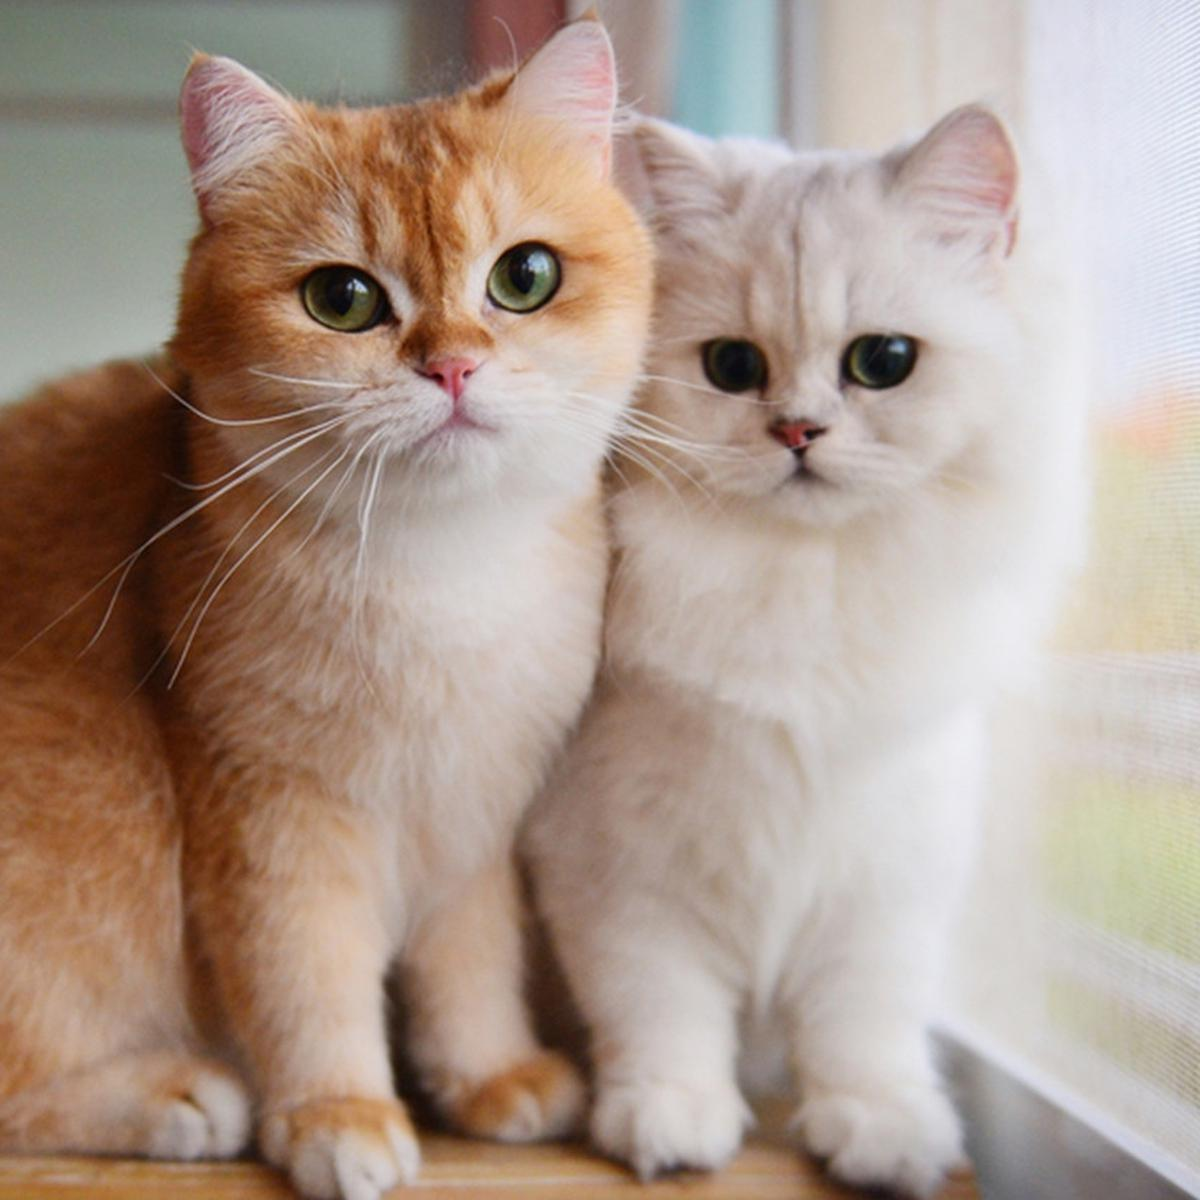
\includegraphics[scale=0.2]{gambar-kucing}
        \caption{Gambar Kucing Lucu dan Imut}
    \end{figure}
\end{lstlisting}

Ukuran gambar dapat diganti dengan mengganti nilai pada scale. Jangan lupa memberikan caption pada setiap gambar. Berikut adalah contoh dari gambar yang telah dimasukkan pada dokumen. Penomoran gambar sudah otomatis dan akan masuk ke daftar gambar juga secara otomatis. Apabila ada beberapa gambar yang akan di embed dengan 1 caption, maka silahkan edit terlebih dahulu dan dijadikan menjadi 1 gambar. Posisi gambar akan pasti setelah dari text ini, apabila ingin mengganti posisinya parameter \textit{H} dapat diganti dengan \textit{h, t, b, p} sesuai kebutuhan.

\begin{figure}[H]
    \centering
    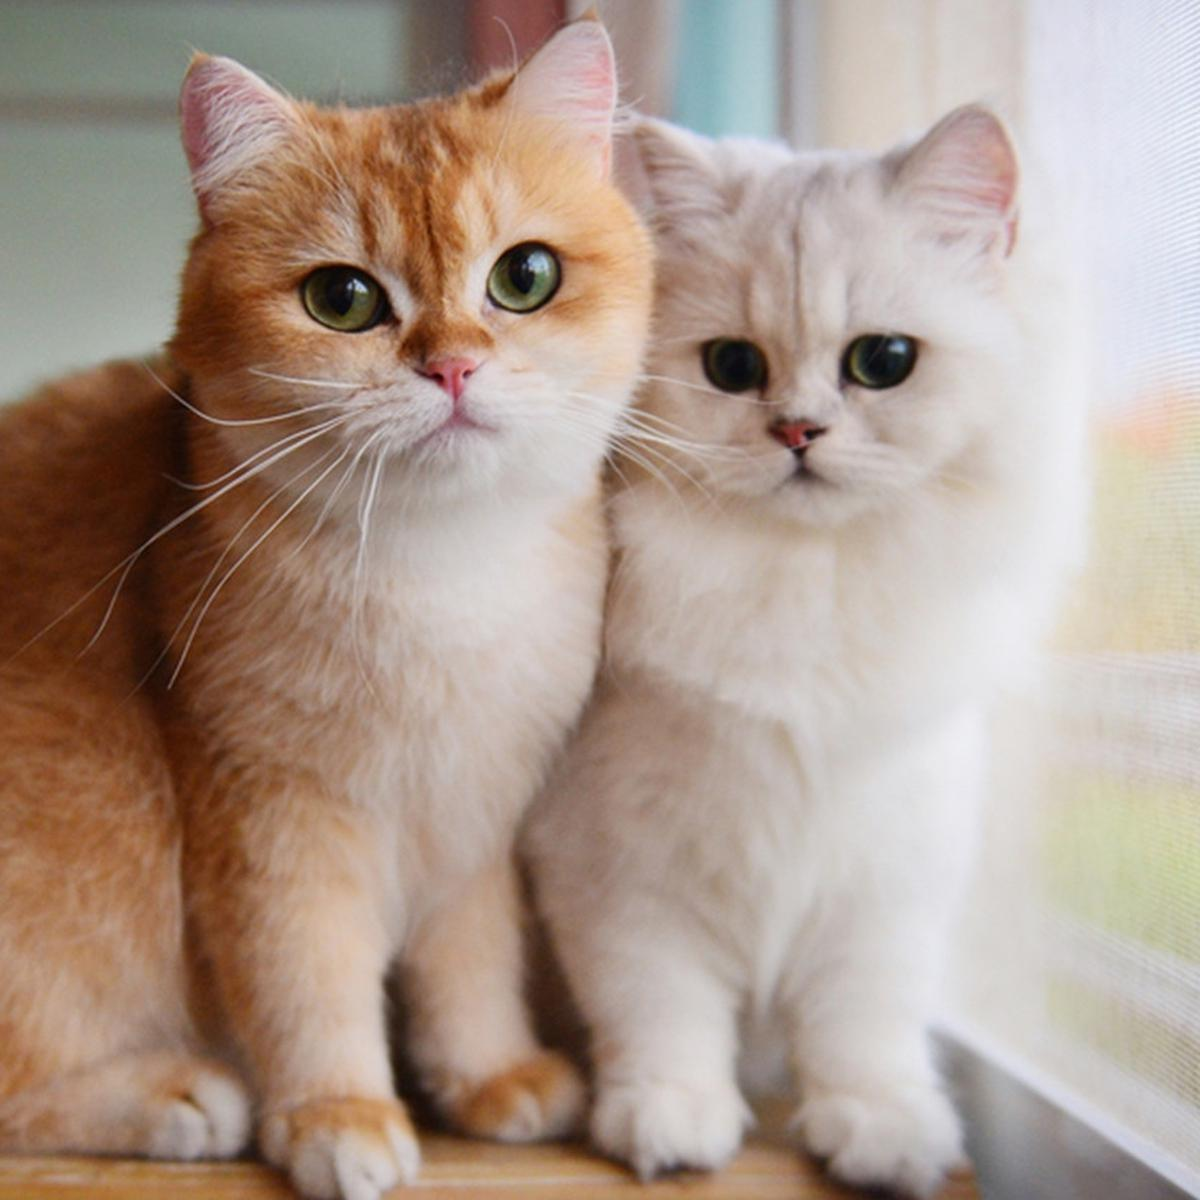
\includegraphics[scale=0.1]{gambar-kucing}
    \caption{Gambar Kucing Lucu dan Imut dengan scala 0.1}
\end{figure}

\begin{figure}[H]
    \centering
    
\includegraphics[scale=0.4]{logo-uny}
    \caption{Logo UNY dengan scala 0.4}
\end{figure}

Untuk menambahkan gambar secara landscape dapat dilihat pada contoh berikut ini.

\begin{sidewaysfigure}[htbp]
	\centering
	
\includegraphics[width=0.6\textwidth]{logo-uny}
	\caption{Logo UNY pada Landscape mode}
\end{sidewaysfigure}

\begin{figure}[H]
    \centering
    \subfigure[]{
     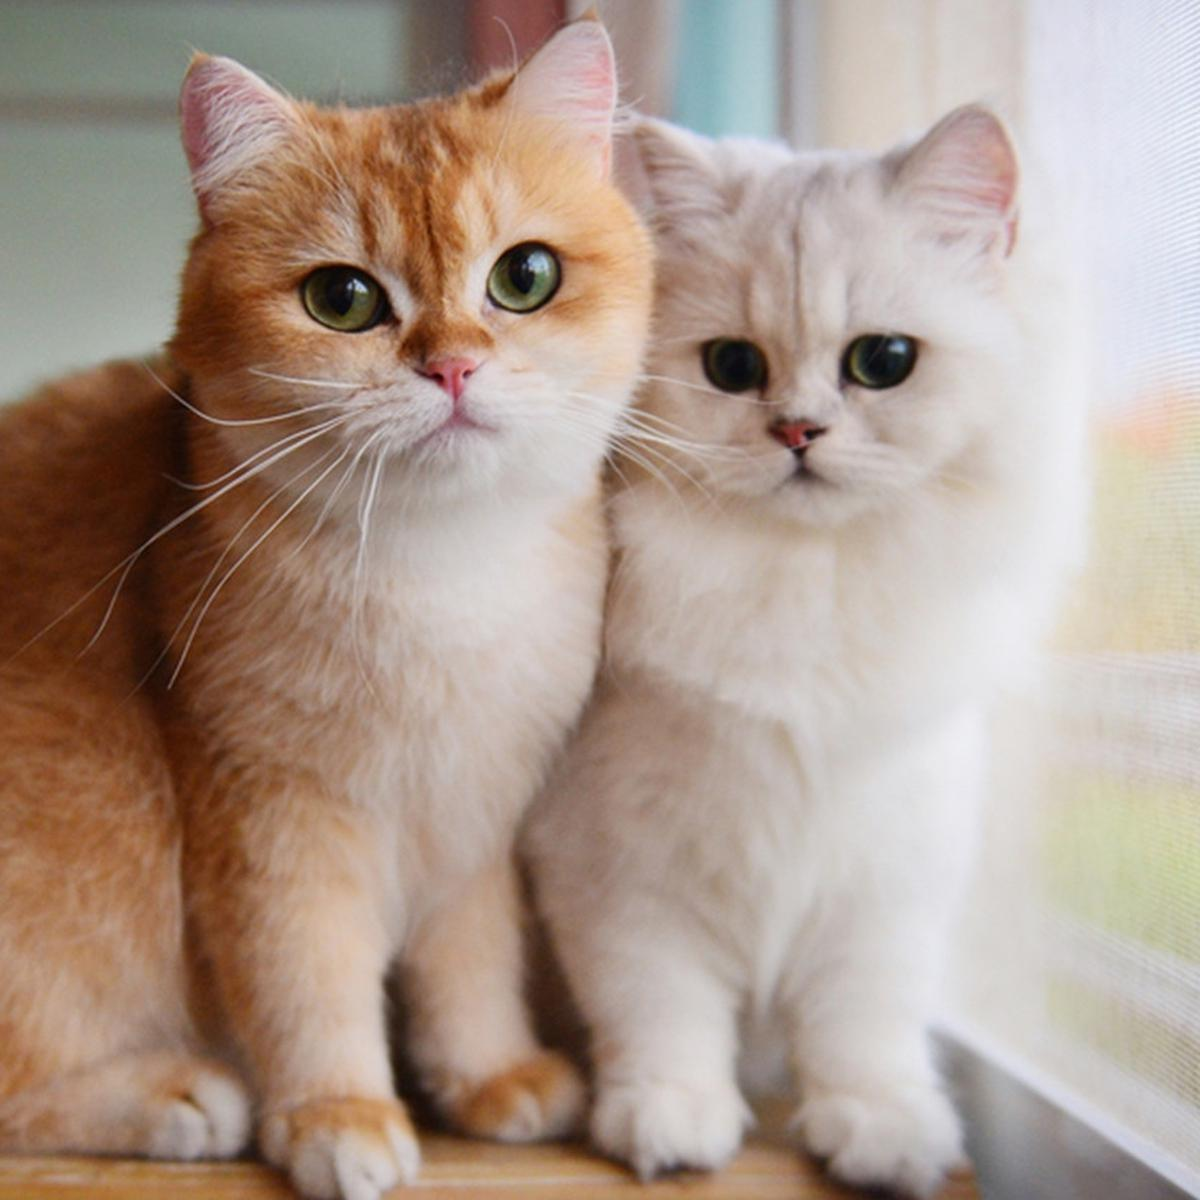
\includegraphics[width=0.4\linewidth]{gambar-kucing}
     }\hspace{0.1\linewidth}
    \subfigure[]{
     
\includegraphics[width=0.4\linewidth]{logo-uny}
    }
    \caption{Dengan menempatkan gambar (a) dan (b), pembaca akan lebih mudah membandingkan keduanya.}
\end{figure}

\subsection{Membuat Tabel}
Pada bagian ini akan dijelaskan bagaimana membuat tabel dalam sebuah dokumen \LaTeX. untuk membuat tabel memang agak sedikit sulit, sehingga saya menyarankan menggunakan tool berikut \url{https://www.tablesgenerator.com/} kemudian isikan tabel pada tool generator tersebut dan salin kodenya ke dalam dokumen \LaTeX. Berikut adalah contoh dari sebuah tabel.

\begin{longtable}{|c|c|}
    \caption{Spesifikasi komputer untuk menjalankan simulator.}
    \label{tb:spesifikasikomputersimulator} \\
    \hline
    OS     & Ubuntu 20.04.2 LTS             \\
    \hline
    Kernel & 5.4.0-80-generic               \\
    \hline
    CPU    & Intel i3-8100 (4) @ 3.600GH    \\
    \hline
    GPU    & NVIDIA GeForce GTX 1050 Ti     \\
    \hline
    RAM    & 7901 MiB                       \\
    \hline
\end{longtable}


Kita juga bisa menambahkan tabel yang besar dengan format halaman landscape seperti contoh berikut.
\begin{sidewaysfigure}[htbp]
	\begin{table}[H]
		\caption{Tabel Sederhana}
		\label{co:tabel}
		\begin{center}
			\begin{tabularx}{0.8\textwidth} {
					|>{\raggedright\arraybackslash}X
					|>{\raggedright\arraybackslash}X
					|>{\raggedright\arraybackslash}X
					|}
				\hline
				$G$     & $\text{dim }G$      & $\text{dim }F$ \\
				\hline
				$SU(N)$ & $N^2 -1$            & $N$            \\
				$SO(N)$ & $\frac{1}{2}N(N-1)$ & $N$            \\
				$Sp(N)$ & $N(2N+1)$           & $2N$           \\
				$E_6$   & $78$                & $27$           \\
				$E_7$   & $133$               & $56$           \\
				$E_8$   & $248$               & $248$          \\
				$F_4$   & $52$                & $6$            \\
				$G_2$   & $14$                & $7$            \\
				\hline
			\end{tabularx}
		\end{center}
	\end{table}
\end{sidewaysfigure}

\begin{table}[H]
	\caption{Tabel Sederhana}
	\label{co:tabel}
	\begin{center}
		\begin{tabularx}{0.8\textwidth} {
				|>{\raggedright\arraybackslash}X
				|>{\raggedright\arraybackslash}X
				|>{\raggedright\arraybackslash}X
				|}
			\hline
			$G$     & $\text{dim }G$      & $\text{dim }F$ \\
			\hline
			$SU(N)$ & $N^2 -1$            & $N$            \\
			$SO(N)$ & $\frac{1}{2}N(N-1)$ & $N$            \\
			$Sp(N)$ & $N(2N+1)$           & $2N$           \\
			$E_6$   & $78$                & $27$           \\
			$E_7$   & $133$               & $56$           \\
			$E_8$   & $248$               & $248$          \\
			$F_4$   & $52$                & $6$            \\
			$G_2$   & $14$                & $7$            \\
			\hline
		\end{tabularx}
	\end{center}
\end{table}

\subsection{Menambahkan listing Kode Program}
Berikut adalah beberapa contoh listing kode yang diembed ke dalam dokumen \LaTeX. kita bisa menentukan bahasa pemrograman yang digunakan, misal seperti python. Berikut adalah contoh dari kode java, python, octave, dan C. Selain itu juga banyak paket yang bisa digunakan untuk styling / highlighting sumber kode yang digunakan, apabila dirasa dibutuhkan bisa ditambahkan manual.

\subsubsection{Java}
Berikut contoh listing kode bahasa pemrograman Java.
\begin{lstlisting}[language=java]
    class HelloWorldApp {
        public static void main(String[] args) {
            System.out.println("Hello World!"); // Display the string.
            for (int i = 0; i < 100; ++i) {
                System.out.println(i);
            }
        }
    }
    \end{lstlisting}

\subsubsection{Python}
Berikut contoh listing kode bahasa pemrograman Python.
\begin{lstlisting}[language=python]
    adj = ["red", "big", "tasty"]
    fruits = ["apple", "banana", "cherry"]

    for x in adj:
        for y in fruits:
            print(x, y)
    \end{lstlisting}

\subsubsection{Octave}
Berikut contoh listing kode bahasa pemrograman Octave.
\begin{lstlisting}[language=octave]
    x = linspace(0, 2*pi, 100);
    y = sin(x);
    plot(x, y);
    figure;
    \end{lstlisting}

\subsubsection{C/C++}
Berikut contoh listing kode bahasa pemrograman C/C++.
\begin{lstlisting}[language=C]
    void setup() {
        Serial.begin(9600);
    }

    void loop() {
        int sensorValue = analogRead(A0);
        Serial.println(sensorValue);
        delay(1);
    }
    \end{lstlisting}

\subsection{Menambahkan Persamaan}
Persamaan tidak lepas dari bidang ilmu teknik dan kadang perlu dituliskan dalam sebuah laporan. Sangat mudah menuliskan persamaan pada sebuah dokumen \LaTeX. Terdapat 2 jenis penulisan persamaan, yaitu inline dengan text seperti contoh ini \(x^2 + y^2 = z^2\) atau seperti ini $E=mc^2$. Jenis lain adalah dituliskan seperti dibawah ini, yang otomatis akan mendapatkan penomoran. Apabila belum familiar dengan kode untuk penulisan persamaan pada \LaTeX bisa menggunakan tool berikut \url{https://latex.codecogs.com/eqneditor/editor.php}.

\begin{equation}
    E=mc^2
\end{equation}

\subsection{Referensi dan Sitasi}
Referensi dan sitasi pada dokumen \LaTeX juga cukup mudah. Silahkan buka file \textit{pustaka.bib} dan amati beberapa contoh penulisan referensi yang ada. Untuk menggenerate bentuk referensi seperti ini dapat menggunakan Mendeley atau Zotero. Mensitasi referensi seperti ini \cite{kongkanand2006} dapat dilakukan dengan perintah \verb|\cite{nama_label}|.

\section{Section 3.3}
Desain dan Implementasi

\subsection{Subsection 3.3.1}
Bagian ini digunakan apabila dibutuhkan, silahkan bisa ditambah atau dikurangi sesuai kebutuhan.

\subsection{Subsection 3.3.2}
Bagian ini digunakan apabila dibutuhkan, silahkan bisa ditambah atau dikurangi sesuai kebutuhan.

\subsection{Subsection 3.3.3}
Bagian ini digunakan apabila dibutuhkan, silahkan bisa ditambah atau dikurangi sesuai kebutuhan.

\section{Section 3.4}
Desain dan Implementasi

\subsection{Subsection 3.4.1}
Bagian ini digunakan apabila dibutuhkan, silahkan bisa ditambah atau dikurangi sesuai kebutuhan.

\subsection{Subsection 3.4.2}
Bagian ini digunakan apabila dibutuhkan, silahkan bisa ditambah atau dikurangi sesuai kebutuhan.

\subsection{Subsection 3.4.3}
Bagian ini digunakan apabila dibutuhkan, silahkan bisa ditambah atau dikurangi sesuai kebutuhan.

\section{Section 3.5}
Section maupun subsection dapat ditambah atau dikurangi sesuai dengan kebutuhan.

\subsection{Subsection 3.5.1}
Bagian ini digunakan apabila dibutuhkan, silahkan bisa ditambah atau dikurangi sesuai kebutuhan.

\subsection{Subsection 3.5.2}
Bagian ini digunakan apabila dibutuhkan, silahkan bisa ditambah atau dikurangi sesuai kebutuhan.

\subsection{Subsection 3.5.3}
Bagian ini digunakan apabila dibutuhkan, silahkan bisa ditambah atau dikurangi sesuai kebutuhan.
\chapter[HASIL DAN PENGUJIAN]{\\ HASIL DAN PENGUJIAN}

\section{Section 4.1}
Hasil adalah bagian dari laporan proyek akhir sarjana terapan yang menjabarkan tentang temuan yang didapat dari pelaksanaan penelitian. Hasil penelitian dapat ditunjukkan dalam bentuk tabel, grafik, atau deskripsi yang menunjukkan data yang didapat dari pengumpulan data. Hasil juga harus dianalisis dan dibahas dalam konteks masalah yang diteliti dan tujuan penelitian.

Dalam laporan proyek akhir sarjana terapan yang meneliti pengaruh perubahan iklim terhadap hasil panen padi, hasil yang didapat dapat ditunjukkan dalam bentuk grafik yang menunjukkan perbandingan hasil panen padi di lokasi yang berbeda dengan kondisi iklim yang berbeda. Hasil ini juga dapat dianalisis dengan menggunakan statistik inferensial untuk mengetahui pengaruh perubahan iklim terhadap hasil panen padi.

Pengujian adalah bagian dari laporan proyek akhir sarjana terapan yang menjabarkan tentang evaluasi dari hasil yang didapat dari pelaksanaan penelitian. Pengujian dilakukan dengan menggunakan metode statistik yang sesuai dengan desain penelitian yang digunakan.

Dalam laporan proyek akhir sarjana terapan yang meneliti pengaruh perubahan iklim terhadap hasil panen padi, pengujian dapat dilakukan dengan menggunakan uji statistik inferensial untuk mengetahui pengaruh perubahan iklim terhadap hasil panen padi. Uji ini dapat dilakukan dengan menggunakan uji-t atau uji-F untuk mengetahui perbedaan yang signifikan antara hasil panen padi di lokasi yang berbeda dengan kondisi iklim yang berbeda.

Hasil dan pengujian dari laporan proyek akhir sarjana terapan harus diinterpretasikan dengan benar dan dibahas dalam konteks masalah yang diteliti dan tujuan penelitian. Selain itu, hasil dan pengujian juga harus dibandingkan dengan hasil penelitian sebelumnya untuk mengetahui keterkaitan dengan penelitian yang telah dilakukan sebelumnya dan memberikan kontribusi baru dalam bidang penelitian terkait.

\subsection{Subsection 4.1.1}
Bagian ini digunakan apabila dibutuhkan, silahkan bisa ditambah atau dikurangi sesuai kebutuhan.

\subsection{Subsection 4.1.2}
Bagian ini digunakan apabila dibutuhkan, silahkan bisa ditambah atau dikurangi sesuai kebutuhan.

\subsection{Subsection 4.1.3}
Bagian ini digunakan apabila dibutuhkan, silahkan bisa ditambah atau dikurangi sesuai kebutuhan.

\section{Section 4.2}
\noindent Hasil dan Pengujian

\subsection{Subsection 4.2.1}
Bagian ini digunakan apabila dibutuhkan, silahkan bisa ditambah atau dikurangi sesuai kebutuhan.

\subsection{Subsection 4.2.2}
Bagian ini digunakan apabila dibutuhkan, silahkan bisa ditambah atau dikurangi sesuai kebutuhan.

\subsection{Subsection 4.2.3}
Bagian ini digunakan apabila dibutuhkan, silahkan bisa ditambah atau dikurangi sesuai kebutuhan.

\section{Section 4.3}
Hasil dan Pengujian

\subsection{Subsection 4.4.1}
Bagian ini digunakan apabila dibutuhkan, silahkan bisa ditambah atau dikurangi sesuai kebutuhan.

\subsection{Subsection 4.4.2}
Bagian ini digunakan apabila dibutuhkan, silahkan bisa ditambah atau dikurangi sesuai kebutuhan.

\subsection{Subsection 4.3.3}
Bagian ini digunakan apabila dibutuhkan, silahkan bisa ditambah atau dikurangi sesuai kebutuhan.

\section{Section 4.4}
Hasil dan Pengujian

\subsection{Subsection 4.4.1}
Bagian ini digunakan apabila dibutuhkan, silahkan bisa ditambah atau dikurangi sesuai kebutuhan.

\subsection{Subsection 4.4.2}
Bagian ini digunakan apabila dibutuhkan, silahkan bisa ditambah atau dikurangi sesuai kebutuhan.

\subsection{Subsection 4.4.3}
Bagian ini digunakan apabila dibutuhkan, silahkan bisa ditambah atau dikurangi sesuai kebutuhan.

\section{Section 4.5}
Hasil dan Pengujian

\subsection{Subsection 4.5.1}
Bagian ini digunakan apabila dibutuhkan, silahkan bisa ditambah atau dikurangi sesuai kebutuhan.

\subsection{Subsection 4.5.2}
Bagian ini digunakan apabila dibutuhkan, silahkan bisa ditambah atau dikurangi sesuai kebutuhan.

\subsection{Subsection 4.5.3}
Bagian ini digunakan apabila dibutuhkan, silahkan bisa ditambah atau dikurangi sesuai kebutuhan.
\chapter[PENUTUP]{\\ PENUTUP}

\section{Kesimpulan}
Kesimpulan adalah bagian penting dari laporan proyek akhir yang menjabarkan tentang temuan yang didapat dari pelaksanaan penelitian dan menjawab masalah yang diteliti sesuai dengan tujuan penelitian. Kesimpulan harus sesuai dengan hasil yang didapat dan dibahas dalam konteks masalah yang diteliti.

Dalam laporan proyek akhir yang meneliti pengaruh perubahan iklim terhadap hasil panen padi, kesimpulan dapat ditarik berdasarkan hasil penelitian yang didapat. Contohnya, jika hasil penelitian menunjukkan bahwa perubahan iklim berpengaruh negatif terhadap hasil panen padi, maka kesimpulan yang dapat ditarik adalah perubahan iklim merupakan faktor yang menurunkan hasil panen padi. Selain itu, kesimpulan juga dapat memberikan saran untuk meningkatkan hasil panen padi yang terdampak oleh perubahan iklim, seperti dengan mengimplementasikan teknologi pertanian yang sesuai atau dengan mengubah pola tanam.

Kesimpulan juga harus dibahas dalam konteks masalah yang diteliti dan tujuan penelitian. Selain itu, kesimpulan juga harus dibandingkan dengan hasil penelitian sebelumnya untuk mengetahui keterkaitan dengan penelitian yang telah dilakukan sebelumnya dan memberikan kontribusi baru dalam bidang penelitian terkait.

Secara keseluruhan, kesimpulan adalah bagian penting dari laporan proyek akhir yang membantu dalam menjabarkan temuan yang didapat dari pelaksanaan penelitian dan menjawab masalah yang diteliti sesuai dengan tujuan penelitian. Kesimpulan harus sesuai dengan hasil yang didapat dan dibahas dalam konteks masalah yang diteliti dan tujuan penelitian. Selain itu, kesimpulan juga harus memberikan saran untuk pengembangan lebih lanjut di bidang yang diteliti dan memberikan kontribusi baru dalam bidang penelitian terkait.

Kesimpulan juga harus dibuat dengan jelas dan ringkas, namun tetap mencakup semua aspek yang diteliti dalam laporan proyek akhir. Selain itu, kesimpulan juga harus dibuat dengan objektif dan tidak mengambil kesimpulan yang tidak didukung oleh data atau hasil penelitian yang didapat.

Secara keseluruhan kesimpulan dari laporan proyek akhir harus memenuhi kriteria yang diharapkan dari laporan proyek akhir yaitu memberikan gambaran yang jelas tentang proses penelitian yang dilakukan, hasil yang didapat, dan kesimpulan yang ditarik serta saran yang diberikan.

\section{Saran}
Saran adalah bagian penting dari laporan proyek akhir yang menjabarkan tentang rekomendasi yang dapat dilakukan untuk pengembangan lebih lanjut dari temuan yang didapat dari pelaksanaan penelitian. Saran harus dibahas dalam konteks masalah yang diteliti dan tujuan penelitian.

Dalam laporan proyek akhir yang meneliti pengaruh perubahan iklim terhadap hasil panen padi, saran dapat diberikan untuk pengembangan lebih lanjut dalam bidang pertanian, seperti:
\begin{packed_item}
    \item Implementasi teknologi pertanian yang sesuai untuk meningkatkan hasil panen padi yang terdampak oleh perubahan iklim
    \item Penelitian lebih lanjut tentang pengaruh perubahan iklim terhadap hasil panen padi di lokasi yang berbeda dengan kondisi iklim yang berbeda
    \item Pembentukan kebijakan pertanian yang sesuai untuk mengatasi masalah perubahan iklim terhadap hasil panen padi
    \item Pendidikan dan sosialisasi tentang perubahan iklim dan cara-cara untuk mengatasinya bagi petani dan masyarakat.
\end{packed_item}

Saran juga harus dibahas dalam konteks masalah yang diteliti dan tujuan penelitian, serta dibandingkan dengan hasil penelitian sebelumnya untuk mengetahui keterkaitan dengan penelitian yang telah dilakukan sebelumnya dan memberikan kontribusi baru dalam bidang penelitian terkait.

Secara keseluruhan, saran adalah bagian penting dari laporan proyek akhir yang membantu dalam memberikan rekomendasi untuk pengembangan lebih lanjut dari temuan yang didapat dari pelaksanaan penelitian. Saran harus dibahas dalam konteks masalah yang diteliti dan tujuan penelitian serta ditujukan untuk memecahkan masalah yang diteliti dan memberikan solusi yang efektif. Saran juga harus dibuat dengan objektif dan tidak berpihak, serta dapat diimplementasikan dalam konteks yang sesuai.
%% DILARANG EDIT BAGIAN INI
\clearpage
\phantomsection
\addcontentsline{toc}{chapter}{DAFTAR PUSTAKA}
\renewcommand\bibname{DAFTAR PUSTAKA}
\nocite{*}
\bibliography{pustaka}
%% DILARANG EDIT BAGIAN INI
\appendix
\chapter*{LAMPIRAN A \\ KODE PROGRAM}
\addcontentsline{toc}{chapter}{LAMPIRAN A KODE PROGRAM}

%isi lampiran kode program disini

\chapter*{LAMPIRAN B \\ GAMBAR-GAMBAR}
\addcontentsline{toc}{chapter}{LAMPIRAN B GAMBAR-GAMBAR}

%isi lampiran gambar-gambar disini

%lampiran ini dapat diedit sesuai kebutuhan, tidak harus lampiran A berisi kode program dan B gambar-gambar
%\chapter*{LAMPIRAN B \\ GAMBAR-GAMBAR}
\addcontentsline{toc}{chapter}{LAMPIRAN B GAMBAR-GAMBAR}
=======
\chapter[PENDAHULUAN]{\\ PENDAHULUAN}

\section{Latar Belakang}
Latar belakang laporan proyek akhir sarjana terapan adalah latar yang menjelaskan tentang alasan dan dasar pemilihan topik proyek akhir, serta permasalahan atau masalah yang akan diteliti dalam proyek tersebut. Latar belakang ini juga menjelaskan tentang bagaimana proyek tersebut dapat memberikan solusi atau kontribusi terhadap permasalahan yang ada.

Proyek akhir sarjana terapan merupakan salah satu syarat untuk menyelesaikan pendidikan sarjana terapan. Proyek ini ditujukan untuk mengaplikasikan ilmu yang didapat dari perkuliahan ke dalam suatu proyek yang sesuai dengan bidang keahlian seseorang. Proyek akhir sarjana terapan juga dapat memberikan kontribusi bagi perkembangan ilmu pengetahuan dan teknologi dalam bidang yang diteliti.

Pemilihan topik proyek akhir sarjana terapan harus sesuai dengan minat dan bidang keahlian seseorang, serta harus memenuhi syarat yang ditentukan oleh institusi pendidikan. Topik yang dipilih harus memiliki permasalahan yang nyata dan dapat memberikan solusi atau kontribusi yang signifikan bagi bidang yang diteliti.

Dalam laporan proyek akhir sarjana terapan, diharapkan dapat diperoleh hasil yang valid dan dapat diuji kembali melalui metode yang sesuai. Hasil yang diperoleh dari proyek ini juga harus dapat memberikan solusi atau kontribusi yang bermanfaat bagi perkembangan ilmu pengetahuan dan teknologi dalam bidang yang diteliti.

Secara keseluruhan, latar belakang laporan proyek akhir sarjana terapan adalah untuk menjelaskan alasan dan dasar pemilihan topik proyek akhir, serta permasalahan atau masalah yang akan diteliti dalam proyek tersebut, serta memberikan solusi atau kontribusi yang bermanfaat bagi perkembangan ilmu pengetahuan dan teknologi dalam bidang yang diteliti.


\section{Rumusan Masalah}
Rumusan masalah dalam laporan proyek akhir sarjana terapan adalah bagian dari laporan yang menjelaskan secara spesifik dan jelas tentang permasalahan atau masalah yang akan diteliti dalam proyek tersebut. Rumusan masalah ini harus dapat diuraikan dengan baik dan jelas sehingga dapat diketahui apa yang akan diteliti dalam proyek akhir sarjana terapan tersebut.

Rumusan masalah dalam laporan proyek akhir sarjana terapan harus ditulis dengan menggunakan kalimat yang jelas dan spesifik. Rumusan masalah harus menjawab pertanyaan "apa yang akan diteliti dalam proyek ini?". Rumusan masalah juga harus memuat permasalahan yang akan diteliti, serta tujuan yang ingin dicapai dari proyek tersebut.

Contoh rumusan masalah dalam laporan proyek akhir sarjana terapan :
"Permasalahan yang akan diteliti dalam proyek ini adalah pengaruh perubahan iklim terhadap produktivitas tanaman padi di wilayah X. Tujuan dari proyek ini adalah untuk mengetahui pengaruh perubahan iklim terhadap produktivitas tanaman padi dan untuk mengetahui cara-cara untuk meningkatkan produktivitas tanaman padi di wilayah X yang terkena dampak perubahan iklim."

Secara keseluruhan, rumusan masalah dalam laporan proyek akhir sarjana terapan adalah bagian dari laporan yang menjelaskan secara jelas dan spesifik tentang permasalahan atau masalah yang akan diteliti dalam proyek tersebut, yang merupakan dasar dari penelitian yang akan dilakukan.

\section{Penelitian Terkait}
Bagian penelitian terkait dalam bab 1 pendahuluan pada laporan proyek akhir sarjana terapan adalah bagian yang menjelaskan tentang studi yang telah dilakukan oleh peneliti sebelumnya yang berhubungan dengan topik yang diteliti dalam proyek akhir sarjana terapan. Bagian ini juga menjelaskan tentang keterkaitan antara hasil penelitian yang telah dilakukan dengan proyek akhir sarjana terapan yang akan dilakukan.

Dalam bagian penelitian terkait, harus dijelaskan tentang studi yang telah dilakukan sebelumnya yang berhubungan dengan topik yang diteliti dalam proyek akhir sarjana terapan, seperti :

\begin{packed_enum}
    \item Judul penelitian
    \item Nama peneliti
    \item Tahun penelitian
    \item Metode penelitian
    \item Hasil penelitian
\end{packed_enum}

Bagian ini juga harus menjelaskan tentang keterkaitan antara hasil penelitian yang telah dilakukan dengan proyek akhir sarjana terapan yang akan dilakukan. Ini akan membantu dalam menjelaskan alasan mengapa proyek akhir sarjana terapan ini penting dan bagaimana proyek ini akan menambah atau menyempurnakan penelitian yang telah dilakukan sebelumnya.

Contoh bagian penelitian terkait dalam bab 1 pendahuluan pada laporan proyek akhir sarjana terapan:
"Beberapa studi telah dilakukan sebelumnya tentang pengaruh perubahan iklim terhadap produktivitas tanaman padi. Penelitian yang dilakukan oleh (nama peneliti) pada tahun (tahun penelitian) menunjukkan bahwa perubahan iklim menyebabkan penurunan produktivitas tanaman padi di wilayah (wilayah penelitian). Penelitian yang dilakukan oleh (nama peneliti) pada tahun (tahun penelitian) menunjukkan bahwa penerapan teknik (teknik yang diterapkan) dapat meningkatkan produktivitas tanaman padi di wilayah yang terkena dampak perubahan iklim. Proyek akhir sarjana terapan ini akan mengevaluasi pengaruh perubahan iklim terhadap produktivitas tanaman padi di wilayah X dan mencari cara-cara untuk meningkatkan produktivitas tanaman padi di wilayah tersebut."

Secara keseluruhan, bagian penelitian terkait dalam bab 1 pendahuluan pada laporan proyek akhir sarjana terapan adalah bagian yang menjelaskan tentang studi yang telah dilakukan oleh peneliti sebelumnya yang berhubungan dengan topik yang diteliti dalam proyek akhir sarjana terapan. Bagian ini bertujuan untuk memberikan gambaran tentang kondisi saat ini dari topik yang diteliti dan membantu dalam menjelaskan alasan mengapa proyek akhir sarjana terapan ini penting dan bagaimana proyek ini akan menambah atau menyempurnakan penelitian yang telah dilakukan sebelumnya. Dengan mengetahui hasil penelitian yang telah dilakukan sebelumnya, peneliti dapat membuat rencana yang lebih baik dan fokus dalam meneliti masalah yang diangkat dalam proyek akhir sarjana terapan.

\section{Tujuan}
Tujuan dalam laporan proyek akhir sarjana terapan adalah bagian yang menjelaskan tentang sasaran yang ingin dicapai dari proyek akhir sarjana terapan yang akan dilakukan. Tujuan ini harus jelas, spesifik, dan dapat diukur. Tujuan dalam laporan proyek akhir sarjana terapan harus menjawab pertanyaan "apa yang ingin dicapai dari proyek ini?"

Tujuan dalam laporan proyek akhir sarjana terapan harus ditulis dengan menggunakan kalimat yang jelas dan spesifik. Tujuan harus dapat diukur dan dapat dicapai melalui metode yang digunakan dalam proyek akhir sarjana terapan. Tujuan juga harus memuat permasalahan yang akan diteliti dan solusi yang akan diberikan melalui proyek akhir sarjana terapan tersebut.

Contoh tujuan dalam laporan proyek akhir sarjana terapan:
"Tujuan dari proyek ini adalah untuk mengetahui pengaruh perubahan iklim terhadap produktivitas tanaman padi di wilayah X dan untuk mengetahui cara-cara untuk meningkatkan produktivitas tanaman padi di wilayah X yang terkena dampak perubahan iklim."

Secara keseluruhan, tujuan dalam laporan proyek akhir sarjana terapan adalah bagian yang menjelaskan tentang sasaran yang ingin dicapai dari proyek akhir sarjana terapan yang akan dilakukan. Tujuan harus jelas, spesifik, dan dapat diukur, serta dapat diperoleh melalui metode yang digunakan dalam proyek akhir sarjana terapan. Tujuan juga harus memuat permasalahan yang akan diteliti dan solusi yang akan diberikan melalui proyek akhir sarjana terapan tersebut.


\section{Batasan Masalah}
Batasan masalah dalam laporan proyek akhir sarjana terapan adalah bagian yang menjelaskan tentang batasan atau keterbatasan dari permasalahan yang diteliti dalam proyek akhir sarjana terapan. Batasan masalah ini harus jelas dan spesifik agar dapat membatasi permasalahan yang diteliti dalam proyek tersebut.

Batasan masalah dalam laporan proyek akhir sarjana terapan harus menjelaskan tentang wilayah atau area yang diteliti, jenis data atau sumber data yang digunakan, metode yang digunakan, serta waktu yang digunakan dalam proyek akhir sarjana terapan.

Contoh batasan masalah dalam laporan proyek akhir sarjana terapan:
"Batasan masalah dalam proyek ini adalah pengaruh perubahan iklim terhadap produktivitas tanaman padi di wilayah X saja. Data yang digunakan dalam proyek ini hanya data yang diperoleh dari observasi lapangan dan wawancara dengan petani tanaman padi di wilayah X. Metode yang digunakan dalam proyek ini hanyalah observasi lapangan dan analisis statistik. Waktu yang digunakan dalam proyek ini adalah selama satu musim tanam."

Secara keseluruhan, batasan masalah dalam laporan proyek akhir sarjana terapan adalah bagian yang menjelaskan tentang batasan atau keterbatasan dari permasalahan yang diteliti dalam proyek akhir sarjana terapan. Batasan masalah harus jelas dan spesifik agar dapat membatasi permasalahan yang diteliti dalam proyek tersebut, seperti wilayah atau area yang diteliti, jenis data atau sumber data yang digunakan, metode yang digunakan, serta waktu yang digunakan dalam proyek akhir sarjana terapan. Ini akan membantu dalam menjelaskan batasan dari proyek yang akan dilakukan dan membuat proyek lebih fokus dalam penelitian.


\section{Sistematika Penulisan}
Sistematika penulisan adalah susunan atau struktur dari laporan proyek akhir sarjana terapan yang menjabarkan bagian-bagian yang harus ada dalam laporan proyek akhir sarjana terapan. Sistematika penulisan dapat berbeda antara satu institusi dengan institusi lainnya, namun umumnya terdiri dari beberapa bagian yang wajib ada, seperti :

\begin{packed_item}
    \item Bab 1 Pendahuluan
    \item Bab 2 Tinjauan Pustaka
    \item Bab 3 Desain dan Implementasi
    \item Bab 4 Hasil dan Pembahasan
    \item Bab 5 Kesimpulan dan Saran
    \item Daftar Pustaka
\end{packed_item}

Penjelasan detail dari masing-masing bab adalah sebagai berikut:

\begin{packed_enum}
    \item Bab 1 Pendahuluan : menjelaskan latar belakang, rumusan masalah, tujuan, batasan masalah, serta sistematika penulisan dari laporan proyek akhir sarjana terapan.
    \item Bab 2 Tinjauan Pustaka : menjabarkan tentang studi yang telah dilakukan oleh peneliti sebelumnya yang berhubungan dengan topik yang diteliti dalam proyek akhir sarjana terapan, serta membahas teori yang relevan dengan masalah yang akan diteliti. Bab ini berisi tentang kajian pustaka yang diperoleh dari berbagai sumber yang terkait dengan masalah yang akan diteliti.
    \item Bab 3 Desain dan Implementasi: menjabarkan tentang rencana dan perencanaan yang digunakan dalam melakukan penelitian dan pelaksanaan penelitian sesuai dengan rencana yang telah ditetapkan dalam desain penelitian. Desain penelitian terdiri dari beberapa elemen, seperti desain penelitian, metode pengumpulan data, sampel, dan analisis data. Implementasi meliputi tahap-tahap dari pelaksanaan penelitian, seperti pengambilan sampel, pengumpulan data, dan analisis data.
    \item Bab 4 Hasil dan Pembahasan: menjabarkan hasil yang diperoleh dari proyek akhir sarjana terapan dan memberikan pembahasan yang mendalam terkait dengan hasil tersebut. Bab ini juga berisi tentang interpretasi data yang diperoleh dari penelitian.
    \item Bab 5 Kesimpulan dan Saran: menjabarkan kesimpulan yang diperoleh dari proyek akhir sarjana terapan serta saran yang diberikan untuk penelitian selanjutnya.
    \item Daftar Pustaka : menjabarkan sumber-sumber yang digunakan dalam laporan proyek akhir sarjana terapan.
\end{packed_enum}

Secara keseluruhan, sistematika penulisan dalam laporan proyek akhir sarjana terapan adalah susunan atau struktur dari laporan proyek akhir sarjana terapan yang menjabarkan bagian-bagian yang harus ada dalam laporan proyek akhir sarjana terapan, yang meliputi Pendahuluan, Tinjauan Pustaka, Metode Penelitian, Hasil dan Pembahasan, Kesimpulan dan Saran, serta Daftar Pustaka. Sistematika penulisan yang baik akan membuat laporan proyek akhir sarjana terapan lebih mudah untuk dibaca dan dipahami.
\chapter[TINJAUAN PUSTAKA]{\\ TINJAUAN PUSTAKA}

\section{Dasar Teori 2.1}
Tinjauan pustaka berdasarkan teori dalam laporan proyek akhir sarjana terapan adalah bagian yang menjabarkan tentang teori yang relevan dengan masalah yang akan diteliti dalam proyek akhir sarjana terapan. Dalam tinjauan pustaka ini, peneliti harus mengumpulkan dan menganalisis sumber-sumber yang berkaitan dengan masalah yang akan diteliti, seperti buku, artikel ilmiah, jurnal, serta sumber-sumber online yang terpercaya.

Dalam tinjauan pustaka berdasarkan teori, peneliti harus menjelaskan :
\begin{packed_item}
    \item Teori-teori yang digunakan dalam penelitian
    \item Konsep-konsep yang digunakan dalam penelitian
    \item Kerangka teori yang digunakan dalam proyek akhir sarjana terapan
\end{packed_item}

Untuk contoh, dalam laporan proyek akhir sarjana terapan yang meneliti pengaruh perubahan iklim terhadap produktivitas tanaman padi, tinjauan pustaka berdasarkan teori harus menjelaskan teori-teori yang digunakan dalam penelitian, seperti teori perubahan iklim, teori produktivitas tanaman, serta teori adaptasi tanaman terhadap perubahan iklim.

Konsep-konsep yang digunakan dalam penelitian, seperti konsep perubahan iklim, konsep produktivitas tanaman, serta konsep adaptasi tanaman terhadap perubahan iklim.

Kerangka teori yang digunakan dalam proyek akhir sarjana terapan harus menjabarkan tentang hubungan antara perubahan iklim, produktivitas tanaman, serta adaptasi tanaman terhadap perubahan iklim.

Selain itu, peneliti juga harus menjelaskan tentang keterkaitan antara teori yang digunakan dengan masalah yang diteliti, dan menjelaskan bagaimana teori tersebut dapat digunakan untuk menjawab masalah yang diteliti.

Secara keseluruhan, Tinjauan pustaka berdasarkan teori dalam laporan proyek akhir sarjana terapan adalah bagian yang menjabarkan tentang teori yang relevan dengan masalah yang akan diteliti dalam proyek akhir sarjana terapan, yang meliputi teori-teori yang digunakan dalam penelitian, konsep-konsep yang digunakan dalam penelitian, serta kerangka teori yang digunakan dalam proyek akhir sarjana terapan. Ini akan membantu dalam menjelaskan konteks dari masalah yang akan diteliti dan bagaimana teori yang digunakan dapat digunakan untuk menjawab masalah tersebut.

Selain itu, tinjauan pustaka berdasarkan teori juga harus menunjukkan keterkaitan antara teori yang digunakan dengan masalah yang diteliti. Hal ini akan membantu dalam menunjukkan validitas teori yang digunakan dalam penelitian dan bagaimana teori tersebut dapat digunakan untuk menjawab masalah yang diteliti.

Tinjauan pustaka berdasarkan teori juga harus menunjukkan keterbatasan dari teori yang digunakan dalam penelitian, seperti keterbatasan dari teori yang digunakan dalam konteks penelitian yang dilakukan. Hal ini akan membantu dalam menunjukkan kelemahan dari teori yang digunakan dan bagaimana teori tersebut dapat diperbaiki atau dikembangkan dalam penelitian selanjutnya.

Dalam keseluruhan, Tinjauan pustaka berdasarkan teori dalam laporan proyek akhir sarjana terapan adalah bagian yang penting dalam menjabarkan teori-teori yang relevan dengan masalah yang akan diteliti dalam proyek akhir sarjana terapan dan membantu dalam menunjukkan konteks dari masalah yang akan diteliti, validitas teori yang digunakan, serta keterbatasan dari teori yang digunakan. Ini akan membantu dalam menyusun dan mengevaluasi penelitian yang dilakukan dan memberikan dasar yang kuat untuk analisis dan pembahasan.

\subsection{Sub Dasar Teori 2.1.1}
Bagian ini digunakan apabila dibutuhkan, silahkan bisa ditambah atau dikurangi sesuai kebutuhan.

\subsection{Sub Dasar Teori 2.1.2}
Bagian ini digunakan apabila dibutuhkan, silahkan bisa ditambah atau dikurangi sesuai kebutuhan.

\subsection{Sub Dasar Teori 2.1.3}
Bagian ini digunakan apabila dibutuhkan, silahkan bisa ditambah atau dikurangi sesuai kebutuhan.

\section{Dasar Teori 2.2}
\noindent Dasar Teori

\subsection{Sub Dasar Teori 2.2.1}
Bagian ini digunakan apabila dibutuhkan, silahkan bisa ditambah atau dikurangi sesuai kebutuhan.

\subsection{Sub Dasar Teori 2.2.2}
Bagian ini digunakan apabila dibutuhkan, silahkan bisa ditambah atau dikurangi sesuai kebutuhan.

\subsection{Sub Dasar Teori 2.2.3}
Bagian ini digunakan apabila dibutuhkan, silahkan bisa ditambah atau dikurangi sesuai kebutuhan.

\section{Dasar Teori 2.3}
Dasar Teori

\subsection{Sub Dasar Teori 2.3.1}
Bagian ini digunakan apabila dibutuhkan, silahkan bisa ditambah atau dikurangi sesuai kebutuhan.

\subsection{Sub Dasar Teori 2.3.2}
Bagian ini digunakan apabila dibutuhkan, silahkan bisa ditambah atau dikurangi sesuai kebutuhan.

\subsection{Sub Dasar Teori 2.3.3}
Bagian ini digunakan apabila dibutuhkan, silahkan bisa ditambah atau dikurangi sesuai kebutuhan.

\section{Dasar Teori 2.4}
Dasar Teori

\subsection{Sub Dasar Teori 2.4.1}
Bagian ini digunakan apabila dibutuhkan, silahkan bisa ditambah atau dikurangi sesuai kebutuhan.

\subsection{Sub Dasar Teori 2.4.2}
Bagian ini digunakan apabila dibutuhkan, silahkan bisa ditambah atau dikurangi sesuai kebutuhan.

\subsection{Sub Dasar Teori 2.4.3}
Bagian ini digunakan apabila dibutuhkan, silahkan bisa ditambah atau dikurangi sesuai kebutuhan.

\section{Dasar Teori 2.5}
\noindent Section maupun subsection dapat ditambah atau dikurangi sesuai dengan kebutuhan.

\subsection{Sub Dasar Teori 2.5.1}
Bagian ini digunakan apabila dibutuhkan, silahkan bisa ditambah atau dikurangi sesuai kebutuhan.

\subsection{Sub Dasar Teori 2.5.2}
Bagian ini digunakan apabila dibutuhkan, silahkan bisa ditambah atau dikurangi sesuai kebutuhan.

\subsection{Sub Dasar Teori 2.5.3}
Bagian ini digunakan apabila dibutuhkan, silahkan bisa ditambah atau dikurangi sesuai kebutuhan.
\chapter[DESAIN DAN IMPLEMENTASI]{\\ DESAIN DAN IMPLEMENTASI}

\section{Section 3.1}
Desain penelitian adalah bagian penting dari laporan proyek akhir sarjana terapan yang menjabarkan tentang rencana dan perencanaan yang digunakan dalam melakukan penelitian. Desain penelitian harus jelas dan terukur, sehingga dapat membantu dalam menjawab masalah yang diteliti. Desain penelitian terdiri dari beberapa elemen, seperti desain penelitian, metode pengumpulan data, sampel, dan analisis data.

Desain penelitian dalam laporan proyek akhir sarjana terapan harus mempertimbangkan beberapa hal, seperti:
\begin{packed_item}
    \item Masalah yang diteliti
    \item Tujuan penelitian
    \item Populasi dan sampel yang digunakan
    \item Metode pengumpulan data
    \item Analisis data yang digunakan
\end{packed_item}

Dalam laporan proyek akhir sarjana terapan yang meneliti pengaruh perubahan iklim terhadap hasil panen padi, desain penelitian yang digunakan adalah desain eksperimen. Desain eksperimen digunakan karena dapat menguji hipotesis dengan mengontrol variabel bebas dan mengukur variabel terikat.

Desain eksperimen ini meliputi pemilihan lokasi penelitian yang sesuai dengan kondisi iklim yang berbeda, pembuatan plot percobaan, dan aplikasi pengaturan iklim yang berbeda pada plot percobaan. Metode pengumpulan data yang dapat digunakan adalah observasi, wawancara dan pengukuran parameter-parameter penting seperti suhu, curah hujan, dan kadar CO2. Sampel yang digunakan adalah tanaman padi yang ditanam di lokasi yang berbeda dengan kondisi iklim yang berbeda. Analisis data yang digunakan adalah statistik deskriptif dan inferensial untuk mengetahui pengaruh perubahan iklim terhadap hasil panen padi.

Implementasi adalah bagian dari laporan proyek akhir sarjana terapan yang menjabarkan tentang pelaksanaan penelitian sesuai dengan rencana yang telah ditetapkan dalam desain penelitian. Implementasi meliputi tahap-tahap dari pelaksanaan penelitian, seperti pengambilan sampel, pengumpulan data, dan analisis data.

Implementasi dari desain penelitian tersebut dilakukan dengan cara mengambil sampel tanaman padi di lokasi yang berbeda dengan kondisi iklim yang berbeda, kemudian melakukan pengukuran parameter-parameter penting seperti suhu, curah hujan, dan kadar CO2. Kemudian data yang didapat dianalisis untuk mengetahui pengaruh perubahan iklim terhadap hasil panen padi.

Dalam proses implementasi, langkah-langkah yang dilakukan meliputi:

\begin{packed_enum}
    \item Pemilihan lokasi penelitian yang sesuai dengan kondisi iklim yang berbeda.
    \item Pembuatan plot percobaan dan pengaturan iklim yang berbeda pada plot percobaan.
    \item Pengambilan sampel tanaman padi di lokasi yang berbeda dengan kondisi iklim yang berbeda.
    \item Pengukuran parameter-parameter penting seperti suhu, curah hujan, dan kadar CO2.
    \item Analisis data yang didapat untuk mengetahui pengaruh perubahan iklim terhadap hasil panen padi.
    \item Implementasi harus dilakukan dengan benar dan teliti agar hasil yang didapat dapat diterima dan dipercaya. Selain itu, implementasi juga harus dilakukan secara objektif agar hasil yang didapat dapat diinterpretasikan dengan benar dan dapat digunakan untuk menjawab masalah yang diteliti.
\end{packed_enum}

Secara keseluruhan, desain dan implementasi adalah bagian penting dari laporan proyek akhir sarjana terapan yang membantu dalam menjabarkan rencana dan pelaksanaan penelitian yang dilakukan. Desain penelitian harus jelas dan terukur serta mempertimbangkan masalah yang diteliti, tujuan penelitian, sampel yang digunakan, metode pengumpulan data, dan analisis data yang digunakan. Implementasi harus dilakukan dengan benar dan teliti serta objektif agar hasil yang didapat dapat diterima dan dipercaya serta dapat digunakan untuk menjawab masalah yang diteliti.

\subsection{Subsection 3.1.1}
Bagian ini digunakan apabila dibutuhkan, silahkan bisa ditambah atau dikurangi sesuai kebutuhan.

\subsection{Subsection 3.1.2}
Bagian ini digunakan apabila dibutuhkan, silahkan bisa ditambah atau dikurangi sesuai kebutuhan.

\subsection{Subsection 3.1.3}
Bagian ini digunakan apabila dibutuhkan, silahkan bisa ditambah atau dikurangi sesuai kebutuhan.

\section{Mengedit dokumen \LaTeX}
Pada bagian ini akan menjelaskan beberapa hal yang diperlukan ketika bekerja pada file \LaTeX.

\subsection{Menambahkan Gambar}
Untuk menambahkan gambar hal yang harus dilakukan adalah:
\begin{packed_enum}
    \item Menyalin file gambar (dalam format jpg \/ png) ke dalam folder \textit{gambar}
    \item Mengganti nama file dari gambar agar mudah dikenali, jangan diberi nama gambar-1,-2, dst
    \item Memasukkan kode di bawah
\end{packed_enum}

\begin{lstlisting}[language=TeX]
    \begin{figure}[H]
        \centering
        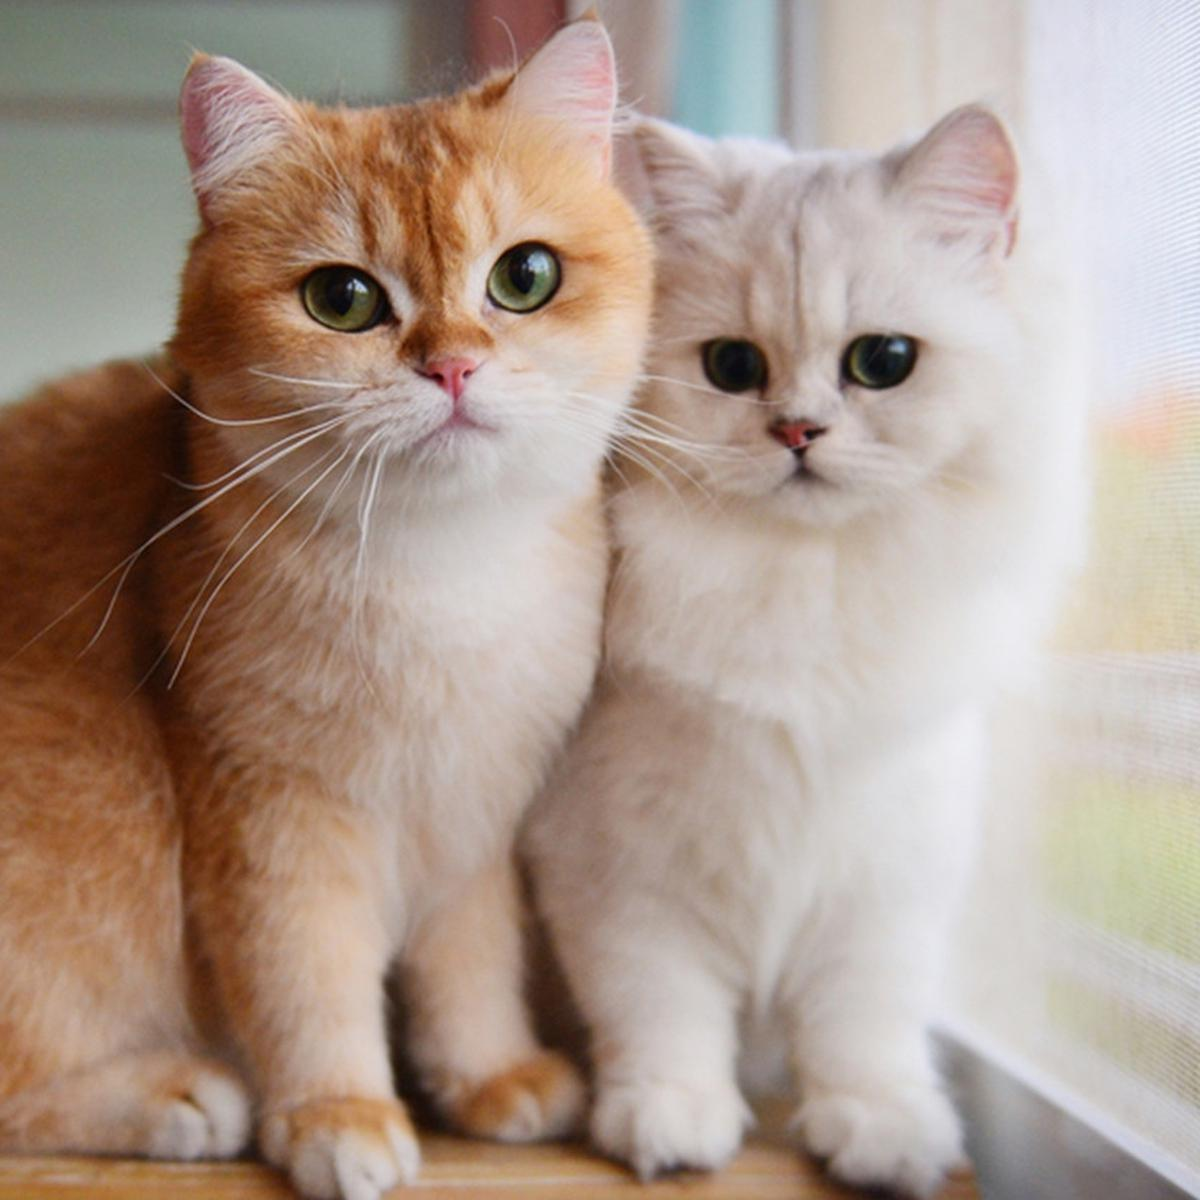
\includegraphics[scale=0.2]{gambar-kucing}
        \caption{Gambar Kucing Lucu dan Imut}
    \end{figure}
\end{lstlisting}

Ukuran gambar dapat diganti dengan mengganti nilai pada scale. Jangan lupa memberikan caption pada setiap gambar. Berikut adalah contoh dari gambar yang telah dimasukkan pada dokumen. Penomoran gambar sudah otomatis dan akan masuk ke daftar gambar juga secara otomatis. Apabila ada beberapa gambar yang akan di embed dengan 1 caption, maka silahkan edit terlebih dahulu dan dijadikan menjadi 1 gambar. Posisi gambar akan pasti setelah dari text ini, apabila ingin mengganti posisinya parameter \textit{H} dapat diganti dengan \textit{h, t, b, p} sesuai kebutuhan.

\begin{figure}[H]
    \centering
    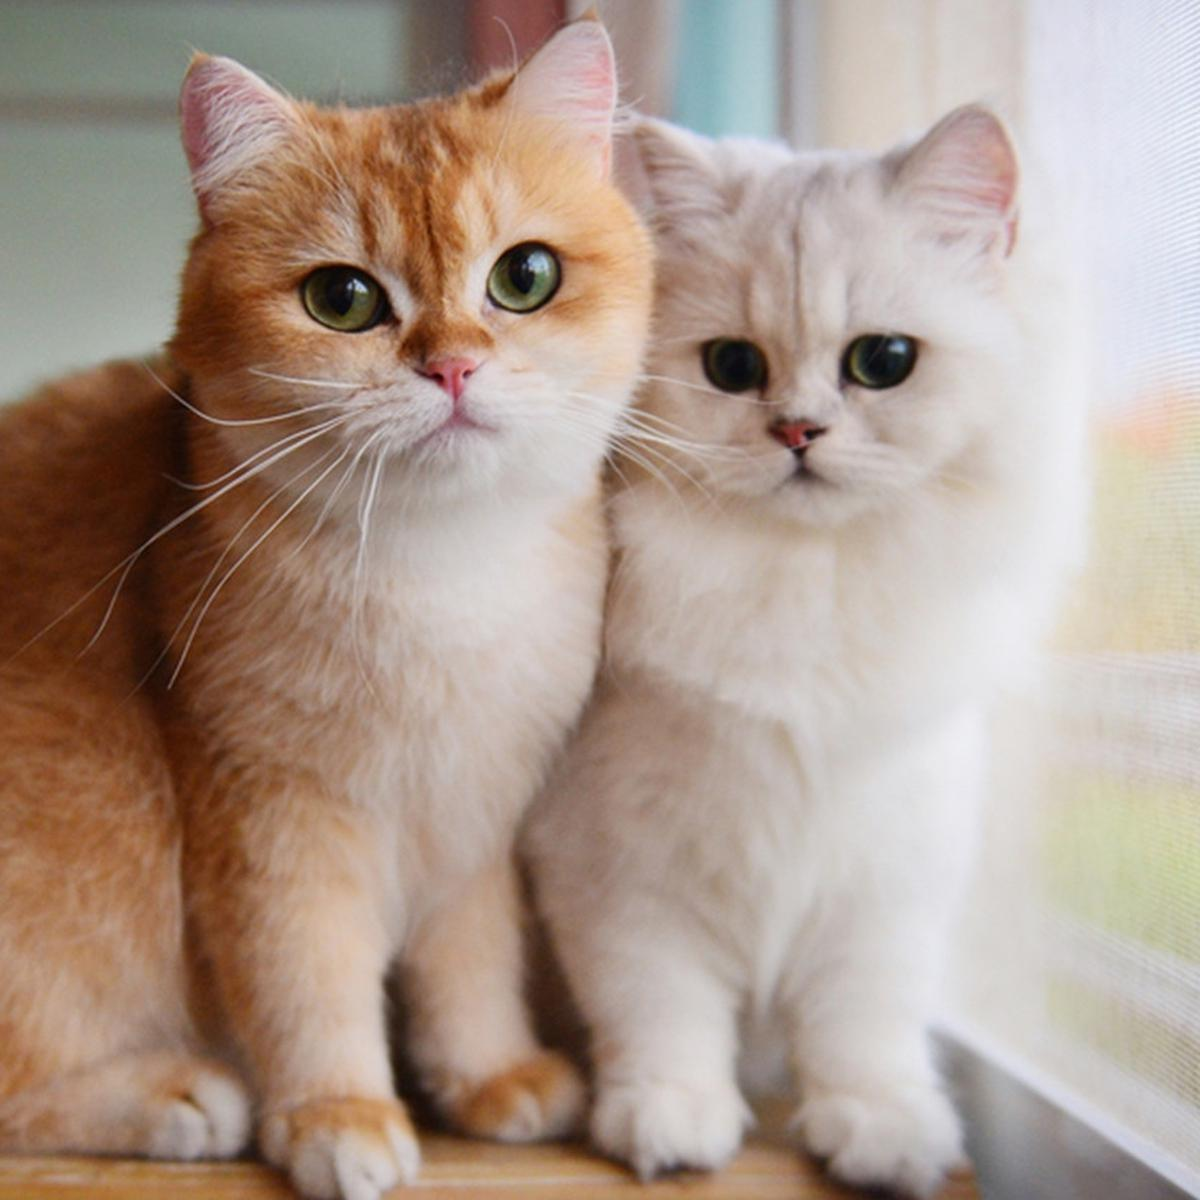
\includegraphics[scale=0.1]{gambar-kucing}
    \caption{Gambar Kucing Lucu dan Imut dengan scala 0.1}
\end{figure}

\begin{figure}[H]
    \centering
    
\includegraphics[scale=0.4]{logo-uny}
    \caption{Logo UNY dengan scala 0.4}
\end{figure}

Untuk menambahkan gambar secara landscape dapat dilihat pada contoh berikut ini.

\begin{sidewaysfigure}[htbp]
	\centering
	
\includegraphics[width=0.6\textwidth]{logo-uny}
	\caption{Logo UNY pada Landscape mode}
\end{sidewaysfigure}

\begin{figure}[H]
    \centering
    \subfigure[]{
     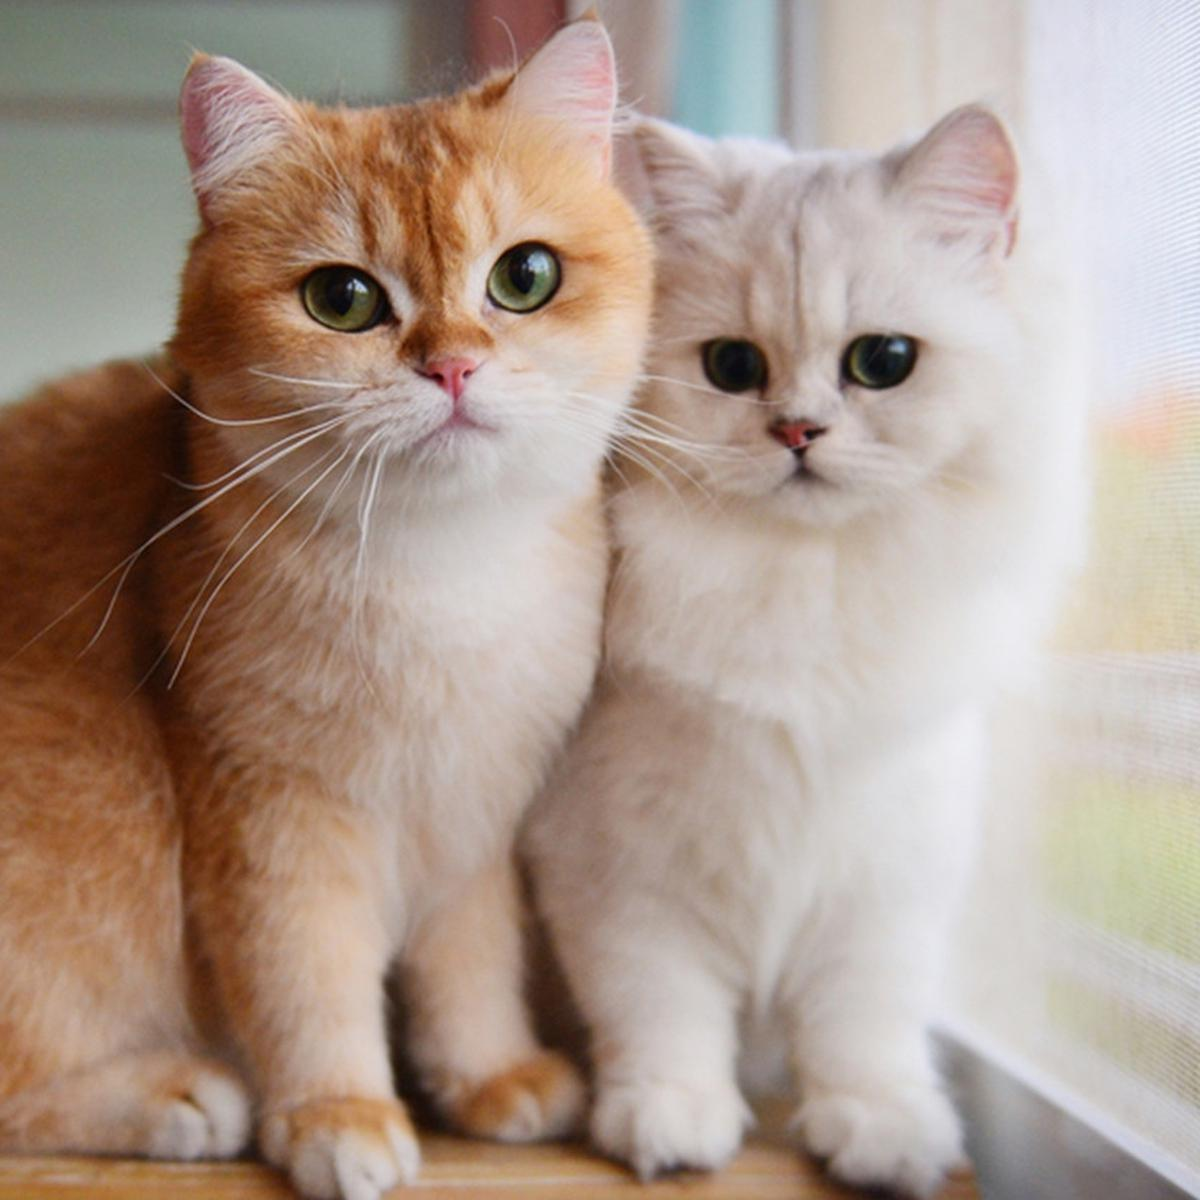
\includegraphics[width=0.4\linewidth]{gambar-kucing}
     }\hspace{0.1\linewidth}
    \subfigure[]{
     
\includegraphics[width=0.4\linewidth]{logo-uny}
    }
    \caption{Dengan menempatkan gambar (a) dan (b), pembaca akan lebih mudah membandingkan keduanya.}
\end{figure}

\subsection{Membuat Tabel}
Pada bagian ini akan dijelaskan bagaimana membuat tabel dalam sebuah dokumen \LaTeX. untuk membuat tabel memang agak sedikit sulit, sehingga saya menyarankan menggunakan tool berikut \url{https://www.tablesgenerator.com/} kemudian isikan tabel pada tool generator tersebut dan salin kodenya ke dalam dokumen \LaTeX. Berikut adalah contoh dari sebuah tabel.

\begin{longtable}{|c|c|}
    \caption{Spesifikasi komputer untuk menjalankan simulator.}
    \label{tb:spesifikasikomputersimulator} \\
    \hline
    OS     & Ubuntu 20.04.2 LTS             \\
    \hline
    Kernel & 5.4.0-80-generic               \\
    \hline
    CPU    & Intel i3-8100 (4) @ 3.600GH    \\
    \hline
    GPU    & NVIDIA GeForce GTX 1050 Ti     \\
    \hline
    RAM    & 7901 MiB                       \\
    \hline
\end{longtable}


Kita juga bisa menambahkan tabel yang besar dengan format halaman landscape seperti contoh berikut.
\begin{sidewaysfigure}[htbp]
	\begin{table}[H]
		\caption{Tabel Sederhana}
		\label{co:tabel}
		\begin{center}
			\begin{tabularx}{0.8\textwidth} {
					|>{\raggedright\arraybackslash}X
					|>{\raggedright\arraybackslash}X
					|>{\raggedright\arraybackslash}X
					|}
				\hline
				$G$     & $\text{dim }G$      & $\text{dim }F$ \\
				\hline
				$SU(N)$ & $N^2 -1$            & $N$            \\
				$SO(N)$ & $\frac{1}{2}N(N-1)$ & $N$            \\
				$Sp(N)$ & $N(2N+1)$           & $2N$           \\
				$E_6$   & $78$                & $27$           \\
				$E_7$   & $133$               & $56$           \\
				$E_8$   & $248$               & $248$          \\
				$F_4$   & $52$                & $6$            \\
				$G_2$   & $14$                & $7$            \\
				\hline
			\end{tabularx}
		\end{center}
	\end{table}
\end{sidewaysfigure}

\begin{table}[H]
	\caption{Tabel Sederhana}
	\label{co:tabel}
	\begin{center}
		\begin{tabularx}{0.8\textwidth} {
				|>{\raggedright\arraybackslash}X
				|>{\raggedright\arraybackslash}X
				|>{\raggedright\arraybackslash}X
				|}
			\hline
			$G$     & $\text{dim }G$      & $\text{dim }F$ \\
			\hline
			$SU(N)$ & $N^2 -1$            & $N$            \\
			$SO(N)$ & $\frac{1}{2}N(N-1)$ & $N$            \\
			$Sp(N)$ & $N(2N+1)$           & $2N$           \\
			$E_6$   & $78$                & $27$           \\
			$E_7$   & $133$               & $56$           \\
			$E_8$   & $248$               & $248$          \\
			$F_4$   & $52$                & $6$            \\
			$G_2$   & $14$                & $7$            \\
			\hline
		\end{tabularx}
	\end{center}
\end{table}

\subsection{Menambahkan listing Kode Program}
Berikut adalah beberapa contoh listing kode yang diembed ke dalam dokumen \LaTeX. kita bisa menentukan bahasa pemrograman yang digunakan, misal seperti python. Berikut adalah contoh dari kode java, python, octave, dan C. Selain itu juga banyak paket yang bisa digunakan untuk styling / highlighting sumber kode yang digunakan, apabila dirasa dibutuhkan bisa ditambahkan manual.

\subsubsection{Java}
Berikut contoh listing kode bahasa pemrograman Java.
\begin{lstlisting}[language=java]
    class HelloWorldApp {
        public static void main(String[] args) {
            System.out.println("Hello World!"); // Display the string.
            for (int i = 0; i < 100; ++i) {
                System.out.println(i);
            }
        }
    }
    \end{lstlisting}

\subsubsection{Python}
Berikut contoh listing kode bahasa pemrograman Python.
\begin{lstlisting}[language=python]
    adj = ["red", "big", "tasty"]
    fruits = ["apple", "banana", "cherry"]

    for x in adj:
        for y in fruits:
            print(x, y)
    \end{lstlisting}

\subsubsection{Octave}
Berikut contoh listing kode bahasa pemrograman Octave.
\begin{lstlisting}[language=octave]
    x = linspace(0, 2*pi, 100);
    y = sin(x);
    plot(x, y);
    figure;
    \end{lstlisting}

\subsubsection{C/C++}
Berikut contoh listing kode bahasa pemrograman C/C++.
\begin{lstlisting}[language=C]
    void setup() {
        Serial.begin(9600);
    }

    void loop() {
        int sensorValue = analogRead(A0);
        Serial.println(sensorValue);
        delay(1);
    }
    \end{lstlisting}

\subsection{Menambahkan Persamaan}
Persamaan tidak lepas dari bidang ilmu teknik dan kadang perlu dituliskan dalam sebuah laporan. Sangat mudah menuliskan persamaan pada sebuah dokumen \LaTeX. Terdapat 2 jenis penulisan persamaan, yaitu inline dengan text seperti contoh ini \(x^2 + y^2 = z^2\) atau seperti ini $E=mc^2$. Jenis lain adalah dituliskan seperti dibawah ini, yang otomatis akan mendapatkan penomoran. Apabila belum familiar dengan kode untuk penulisan persamaan pada \LaTeX bisa menggunakan tool berikut \url{https://latex.codecogs.com/eqneditor/editor.php}.

\begin{equation}
    E=mc^2
\end{equation}

\subsection{Referensi dan Sitasi}
Referensi dan sitasi pada dokumen \LaTeX juga cukup mudah. Silahkan buka file \textit{pustaka.bib} dan amati beberapa contoh penulisan referensi yang ada. Untuk menggenerate bentuk referensi seperti ini dapat menggunakan Mendeley atau Zotero. Mensitasi referensi seperti ini \cite{kongkanand2006} dapat dilakukan dengan perintah \verb|\cite{nama_label}|.

\section{Section 3.3}
Desain dan Implementasi

\subsection{Subsection 3.3.1}
Bagian ini digunakan apabila dibutuhkan, silahkan bisa ditambah atau dikurangi sesuai kebutuhan.

\subsection{Subsection 3.3.2}
Bagian ini digunakan apabila dibutuhkan, silahkan bisa ditambah atau dikurangi sesuai kebutuhan.

\subsection{Subsection 3.3.3}
Bagian ini digunakan apabila dibutuhkan, silahkan bisa ditambah atau dikurangi sesuai kebutuhan.

\section{Section 3.4}
Desain dan Implementasi

\subsection{Subsection 3.4.1}
Bagian ini digunakan apabila dibutuhkan, silahkan bisa ditambah atau dikurangi sesuai kebutuhan.

\subsection{Subsection 3.4.2}
Bagian ini digunakan apabila dibutuhkan, silahkan bisa ditambah atau dikurangi sesuai kebutuhan.

\subsection{Subsection 3.4.3}
Bagian ini digunakan apabila dibutuhkan, silahkan bisa ditambah atau dikurangi sesuai kebutuhan.

\section{Section 3.5}
Section maupun subsection dapat ditambah atau dikurangi sesuai dengan kebutuhan.

\subsection{Subsection 3.5.1}
Bagian ini digunakan apabila dibutuhkan, silahkan bisa ditambah atau dikurangi sesuai kebutuhan.

\subsection{Subsection 3.5.2}
Bagian ini digunakan apabila dibutuhkan, silahkan bisa ditambah atau dikurangi sesuai kebutuhan.

\subsection{Subsection 3.5.3}
Bagian ini digunakan apabila dibutuhkan, silahkan bisa ditambah atau dikurangi sesuai kebutuhan.
\chapter[HASIL DAN PENGUJIAN]{\\ HASIL DAN PENGUJIAN}

\section{Section 4.1}
Hasil adalah bagian dari laporan proyek akhir sarjana terapan yang menjabarkan tentang temuan yang didapat dari pelaksanaan penelitian. Hasil penelitian dapat ditunjukkan dalam bentuk tabel, grafik, atau deskripsi yang menunjukkan data yang didapat dari pengumpulan data. Hasil juga harus dianalisis dan dibahas dalam konteks masalah yang diteliti dan tujuan penelitian.

Dalam laporan proyek akhir sarjana terapan yang meneliti pengaruh perubahan iklim terhadap hasil panen padi, hasil yang didapat dapat ditunjukkan dalam bentuk grafik yang menunjukkan perbandingan hasil panen padi di lokasi yang berbeda dengan kondisi iklim yang berbeda. Hasil ini juga dapat dianalisis dengan menggunakan statistik inferensial untuk mengetahui pengaruh perubahan iklim terhadap hasil panen padi.

Pengujian adalah bagian dari laporan proyek akhir sarjana terapan yang menjabarkan tentang evaluasi dari hasil yang didapat dari pelaksanaan penelitian. Pengujian dilakukan dengan menggunakan metode statistik yang sesuai dengan desain penelitian yang digunakan.

Dalam laporan proyek akhir sarjana terapan yang meneliti pengaruh perubahan iklim terhadap hasil panen padi, pengujian dapat dilakukan dengan menggunakan uji statistik inferensial untuk mengetahui pengaruh perubahan iklim terhadap hasil panen padi. Uji ini dapat dilakukan dengan menggunakan uji-t atau uji-F untuk mengetahui perbedaan yang signifikan antara hasil panen padi di lokasi yang berbeda dengan kondisi iklim yang berbeda.

Hasil dan pengujian dari laporan proyek akhir sarjana terapan harus diinterpretasikan dengan benar dan dibahas dalam konteks masalah yang diteliti dan tujuan penelitian. Selain itu, hasil dan pengujian juga harus dibandingkan dengan hasil penelitian sebelumnya untuk mengetahui keterkaitan dengan penelitian yang telah dilakukan sebelumnya dan memberikan kontribusi baru dalam bidang penelitian terkait.

\subsection{Subsection 4.1.1}
Bagian ini digunakan apabila dibutuhkan, silahkan bisa ditambah atau dikurangi sesuai kebutuhan.

\subsection{Subsection 4.1.2}
Bagian ini digunakan apabila dibutuhkan, silahkan bisa ditambah atau dikurangi sesuai kebutuhan.

\subsection{Subsection 4.1.3}
Bagian ini digunakan apabila dibutuhkan, silahkan bisa ditambah atau dikurangi sesuai kebutuhan.

\section{Section 4.2}
\noindent Hasil dan Pengujian

\subsection{Subsection 4.2.1}
Bagian ini digunakan apabila dibutuhkan, silahkan bisa ditambah atau dikurangi sesuai kebutuhan.

\subsection{Subsection 4.2.2}
Bagian ini digunakan apabila dibutuhkan, silahkan bisa ditambah atau dikurangi sesuai kebutuhan.

\subsection{Subsection 4.2.3}
Bagian ini digunakan apabila dibutuhkan, silahkan bisa ditambah atau dikurangi sesuai kebutuhan.

\section{Section 4.3}
Hasil dan Pengujian

\subsection{Subsection 4.4.1}
Bagian ini digunakan apabila dibutuhkan, silahkan bisa ditambah atau dikurangi sesuai kebutuhan.

\subsection{Subsection 4.4.2}
Bagian ini digunakan apabila dibutuhkan, silahkan bisa ditambah atau dikurangi sesuai kebutuhan.

\subsection{Subsection 4.3.3}
Bagian ini digunakan apabila dibutuhkan, silahkan bisa ditambah atau dikurangi sesuai kebutuhan.

\section{Section 4.4}
Hasil dan Pengujian

\subsection{Subsection 4.4.1}
Bagian ini digunakan apabila dibutuhkan, silahkan bisa ditambah atau dikurangi sesuai kebutuhan.

\subsection{Subsection 4.4.2}
Bagian ini digunakan apabila dibutuhkan, silahkan bisa ditambah atau dikurangi sesuai kebutuhan.

\subsection{Subsection 4.4.3}
Bagian ini digunakan apabila dibutuhkan, silahkan bisa ditambah atau dikurangi sesuai kebutuhan.

\section{Section 4.5}
Hasil dan Pengujian

\subsection{Subsection 4.5.1}
Bagian ini digunakan apabila dibutuhkan, silahkan bisa ditambah atau dikurangi sesuai kebutuhan.

\subsection{Subsection 4.5.2}
Bagian ini digunakan apabila dibutuhkan, silahkan bisa ditambah atau dikurangi sesuai kebutuhan.

\subsection{Subsection 4.5.3}
Bagian ini digunakan apabila dibutuhkan, silahkan bisa ditambah atau dikurangi sesuai kebutuhan.
\chapter[PENUTUP]{\\ PENUTUP}

\section{Kesimpulan}
Kesimpulan adalah bagian penting dari laporan proyek akhir yang menjabarkan tentang temuan yang didapat dari pelaksanaan penelitian dan menjawab masalah yang diteliti sesuai dengan tujuan penelitian. Kesimpulan harus sesuai dengan hasil yang didapat dan dibahas dalam konteks masalah yang diteliti.

Dalam laporan proyek akhir yang meneliti pengaruh perubahan iklim terhadap hasil panen padi, kesimpulan dapat ditarik berdasarkan hasil penelitian yang didapat. Contohnya, jika hasil penelitian menunjukkan bahwa perubahan iklim berpengaruh negatif terhadap hasil panen padi, maka kesimpulan yang dapat ditarik adalah perubahan iklim merupakan faktor yang menurunkan hasil panen padi. Selain itu, kesimpulan juga dapat memberikan saran untuk meningkatkan hasil panen padi yang terdampak oleh perubahan iklim, seperti dengan mengimplementasikan teknologi pertanian yang sesuai atau dengan mengubah pola tanam.

Kesimpulan juga harus dibahas dalam konteks masalah yang diteliti dan tujuan penelitian. Selain itu, kesimpulan juga harus dibandingkan dengan hasil penelitian sebelumnya untuk mengetahui keterkaitan dengan penelitian yang telah dilakukan sebelumnya dan memberikan kontribusi baru dalam bidang penelitian terkait.

Secara keseluruhan, kesimpulan adalah bagian penting dari laporan proyek akhir yang membantu dalam menjabarkan temuan yang didapat dari pelaksanaan penelitian dan menjawab masalah yang diteliti sesuai dengan tujuan penelitian. Kesimpulan harus sesuai dengan hasil yang didapat dan dibahas dalam konteks masalah yang diteliti dan tujuan penelitian. Selain itu, kesimpulan juga harus memberikan saran untuk pengembangan lebih lanjut di bidang yang diteliti dan memberikan kontribusi baru dalam bidang penelitian terkait.

Kesimpulan juga harus dibuat dengan jelas dan ringkas, namun tetap mencakup semua aspek yang diteliti dalam laporan proyek akhir. Selain itu, kesimpulan juga harus dibuat dengan objektif dan tidak mengambil kesimpulan yang tidak didukung oleh data atau hasil penelitian yang didapat.

Secara keseluruhan kesimpulan dari laporan proyek akhir harus memenuhi kriteria yang diharapkan dari laporan proyek akhir yaitu memberikan gambaran yang jelas tentang proses penelitian yang dilakukan, hasil yang didapat, dan kesimpulan yang ditarik serta saran yang diberikan.

\section{Saran}
Saran adalah bagian penting dari laporan proyek akhir yang menjabarkan tentang rekomendasi yang dapat dilakukan untuk pengembangan lebih lanjut dari temuan yang didapat dari pelaksanaan penelitian. Saran harus dibahas dalam konteks masalah yang diteliti dan tujuan penelitian.

Dalam laporan proyek akhir yang meneliti pengaruh perubahan iklim terhadap hasil panen padi, saran dapat diberikan untuk pengembangan lebih lanjut dalam bidang pertanian, seperti:
\begin{packed_item}
    \item Implementasi teknologi pertanian yang sesuai untuk meningkatkan hasil panen padi yang terdampak oleh perubahan iklim
    \item Penelitian lebih lanjut tentang pengaruh perubahan iklim terhadap hasil panen padi di lokasi yang berbeda dengan kondisi iklim yang berbeda
    \item Pembentukan kebijakan pertanian yang sesuai untuk mengatasi masalah perubahan iklim terhadap hasil panen padi
    \item Pendidikan dan sosialisasi tentang perubahan iklim dan cara-cara untuk mengatasinya bagi petani dan masyarakat.
\end{packed_item}

Saran juga harus dibahas dalam konteks masalah yang diteliti dan tujuan penelitian, serta dibandingkan dengan hasil penelitian sebelumnya untuk mengetahui keterkaitan dengan penelitian yang telah dilakukan sebelumnya dan memberikan kontribusi baru dalam bidang penelitian terkait.

Secara keseluruhan, saran adalah bagian penting dari laporan proyek akhir yang membantu dalam memberikan rekomendasi untuk pengembangan lebih lanjut dari temuan yang didapat dari pelaksanaan penelitian. Saran harus dibahas dalam konteks masalah yang diteliti dan tujuan penelitian serta ditujukan untuk memecahkan masalah yang diteliti dan memberikan solusi yang efektif. Saran juga harus dibuat dengan objektif dan tidak berpihak, serta dapat diimplementasikan dalam konteks yang sesuai.
\clearpage
\phantomsection
\addcontentsline{toc}{chapter}{DAFTAR PUSTAKA}
\renewcommand\bibname{DAFTAR PUSTAKA}
\nocite{*}
\bibliography{pustaka}
\appendix
\chapter*{LAMPIRAN A \\ KODE PROGRAM}
\addcontentsline{toc}{chapter}{LAMPIRAN A KODE PROGRAM}

%isi lampiran kode program disini

\chapter*{LAMPIRAN B \\ GAMBAR-GAMBAR}
\addcontentsline{toc}{chapter}{LAMPIRAN B GAMBAR-GAMBAR}

%isi lampiran gambar-gambar disini

%lampiran ini dapat diedit sesuai kebutuhan, tidak harus lampiran A berisi kode program dan B gambar-gambar
>>>>>>> 37411a41c51b7cb35cb8691317ba382e7dca4495
\end{document}